% ----------------------------------- 
% TODO : modifié ce début de fichier 
% 
% Ce dossier de spécification est fortement inspiré du dossier de spécification réalisé par Milo KOSON de l'année dernière
%
% Document modifié et adapté par Théo BENARD
%-----------------------------------
\documentclass[a4paper,11pt,titlepage,french]{article}
% classe de document pour LaTeX qui définit les paramètres généraux du document : 
    % a4paper : définit le format de papier sur lequel le document doit être imprimé (a4paper format standard)
    % 11pt : définit la taille de police de base à 11 points
    % titlepage : demande à LaTeX d'insérer une page de titre dans le document
    % french : Cette option indique à LaTeX que le document est rédigé en français
% TODO : \input{chemin vers le fichier de setup} 
    % le fichier de setup devra contenir l'ensemble des usepackage suivants et les variables globales
% ----------------
% LIBRAIRIES LATEX
% ----------------
\usepackage[main=french]{babel}
\usepackage[T1]{fontenc}
\usepackage{fontspec}
\usepackage{fancyhdr}
\usepackage{xspace, graphicx}
\usepackage{longtable}
\usepackage[table]{xcolor}
\usepackage{hyperref}
\usepackage{enumitem}

\usepackage{caption}
\usepackage{lastpage}

%\usepackage[outdir=build/epstopdf/, update]{epstopdf}
%\usepackage{array}
%\usepackage{multirow}
%\usepackage{changepage}
%\usepackage{hyperref}
%\usepackage{refcount}
% ------------------
% VARIABLES GLOBALES
% ------------------
\newcommand{\version}{2.0}
\newcommand{\revision}{0}
\newcommand{\documentName}{Dossier de Spécifications}
\newcommand{\documentNameAbrev}{SPEC}
\newcommand{\prose}{ProSE}
\newcommand{\creator}{Théo BENARD}
\newcommand{\projectName}{Passerelle Android-CAN vers banc CAN réel ou simulé} % TODO
\newcommand{\annee}{2024}
\newcommand{\teamName}{CANvengers} 
\newcommand{\teamNumber}{B1}
\newcommand{\client}{KEREVAL}
\newcommand{\nomLogiciel}{CANgateway} 
\newcommand{\nomApplication}{CANdroid} 

\setcounter{secnumdepth}{4} % Pour avoir une numérotation jusqu'au niveau 4
\renewcommand{\theparagraph}{\thesubsubsection.\arabic{paragraph}} % Pour numéroter les paragraphes à partir du niveau 3
\makeatletter % Redéfinit la commande \paragraph pour qu'elle utilise les paramètres de formatage de la commande \subsubsection.
\renewcommand\paragraph{\@startsection{paragraph}{4}{\z@}%
    {-3.25ex \@plus -1ex \@minus -.2ex}%
    {1.5ex \@plus .2ex}%
    {\normalfont\normalsize\bfseries}}
\makeatother

% -------------------------------------------------------
% --------------------------
% PARAMETRES HEADER / FOOTER 
% --------------------------
\pagestyle{fancy} % permet de personnaliser l'apparence de l'en-tête et du pied de page de chaque page du document
\setlength{\hoffset}{-40pt} % définis la marge horizontale gauche
\setlength{\topmargin}{-25pt} % définis la marge supérieure 
\setlength{\headsep}{10pt} % définis l'espace vertical entre l'en-tête et le corps de texte 
\renewcommand{\headheight}{60pt} % redéfinis la hauteur de l'en-tête
\renewcommand{\headwidth}{450pt} %  redéfinis la largeur de l'en-tête
\setlength{\textwidth}{450pt} % définis la largeur du corps de texte
\setlength{\textheight}{604pt} %  définis la hauteur du corps de texte
\renewcommand{\footrulewidth}{0.1mm} % redéfinis la largeur de la ligne de séparation de pied de page
\fancyhf{} % vide les entêtes et pieds de page précédemment définis
    % HEADER %
    \fancyhead[LO]{\bf \includegraphics[width=80pt]{../figures/eseo.png}\\ % fancyhead - personnaliser l'en-tête avec 2 arguments : orientation "LO" pour "Left Odd" / contenu "\bf" pour texte en gras + "\includegraphics" inclure le logo de l'ESEO
        \medskip % ajoute espace vertical moyen (≃ 6 points)
        {\prose} équipe {\teamNumber} {\annee}} % texte en dessous de l'image de la partie gauche du pdf
    \fancyhead[RO]{\bf 
\includegraphics[width=90pt]{../figures/logo_kereval.png}\\ % fancyhead - personnaliser l'en-tête avec 2 arguments : orientation "RO" pour "Right Odd" / contenu "\bf" pour texte en gras + "\includegraphics" inclure le logo de l'entreprise
        {\small{Ref. {\documentNameAbrev}\_{\teamNumber}}}} % texte en dessous de l'image de la partie droite du pdf
    % FOOTER %
    \fancyfoot[LO]{\sl {\it Version {\version} - Révision {\revision}}} % fancyfoot - personnaliser le pied de page avec 2 arguments : position "LO" pour "Left Odd" / contenu "\sl" + "\it" pour texte en italique de la version et la révision
    \cfoot{\copyright {\annee} Droits réservés {\teamName}} % insérer texte au centre du pied de page
    \fancyfoot[RO]{\thepage/\pageref{LastPage}} % pied de page partie droite : numéro de page
% ------------------------------
% FIN PARAMETRES HEADER / FOOTER 
% ------------------------------
% --------------
% DEBUT DOCUMENT 
% --------------
\begin{document}
\sloppy % relâche les règles de justification de texte pour éviter des espaces trop larges
\renewcommand{\arraystretch}{1.3} % augmente la hauteur des lignes d'un tableau

%-----------------------------------------------
%   The titles of the parts
%-----------------------------------------------
\makeatletter
% Adds a sub-subparagraph level
\newcounter{subsubparagraph}[subparagraph]
\renewcommand\thesubsubparagraph{%
    \thesubparagraph.\@arabic\c@subsubparagraph}
\newcommand\subsubparagraph{%
    \@startsection{subsubparagraph}               % counter
    {6}                                           % level
    {0em}                                         % indentation
    {1em}                                         % before the title
    {1em}                                         % after the title
    {\normalsize\hspace{6em}\color{colorTitle}} % style (overloaded by the title format)
}
\newcommand\l@subsubparagraph{\@dottedtocline{6}{13em}{6em}}
\newcommand{\subsubparagraphmark}[1]{}
\providecommand*{\toclevel@subsubparagraph}{6}

\setcounter{tocdepth}{6}    % Allows the paragraph in the table of contents
\setcounter{secnumdepth}{6} % Allows the numbering of the sub-paragraph

\makeatother
% -------------------
% PAGE DE GARDE {p.1}
% -------------------
\begin{center} % centre le contenu de la commande
    \vspace*{2cm} % ajout d'espace
    \rule[0.5ex]{0.7\textwidth}{0.1mm}\\ % ajout ligne horizontale : décalage verticale "ex" / largeur de page "%" / épaisseur "mm"
    \vspace*{2mm} % ajout d'espace
        {\Huge {\textsc{\bf {\documentName}}}} % crée un titre : police en gras "\bf" / petites capitales "\textsc" / grande taille polile "\Huge" 
    \vspace{0.4cm}\\ % ajout d'espace / "\\" : retour à la ligne 
        {\large\bf {\prose} {\teamNumber} {\annee} - {\teamName}}\\ % crée un titre : police en gras "\bf" / taille de police relativement grande "\large"
    \vspace*{1mm}
        {\large\bf {\projectName}}\\ % crée un titre 
    \rule[0.5ex]{0.75\textwidth}{0.1mm}\\ % ajout ligne horizontale
    \vspace{2cm} 
    \begin{tabular}{|c|c|} % crée un tableau avec 2 colonnes 
        \hline % crée une ligne dans le tableau // & : séparateur colonne
            Responsable du document & {\creator}                      \\
            État du document        & Validé                          \\
            Version                 & {\version}                      \\
            Révision                & {\revision}                     \\
        \hline
    \end{tabular}
\end{center}
\vspace{3cm} 
% -------------------
% AVERTISSEMENT {p.1}
% -------------------
\noindent % supprime l'indentation automatique au début d'un paragraphe
\textbf{AVERTISSEMENT :} % titre avertissement en gras
\vspace{3mm} \\
Le présent document est un document à but pédagogique.  
Le document de conception ci-joint est strictement confidentiel et réservé à un usage interne. 
Il a été réalisé sous la direction de Jérôme DELATOUR, en collaboration avec des enseignants 
et des étudiants de l'option SE du groupe ESEO. Ce document est la propriété de Jérôme DELATOUR, du groupe ESEO.
Toute utilisation, diffusion ou reproduction de ce document sans autorisation écrite préalable de Jérôme DELATOUR est interdite. 
Nous tenons à souligner que toute violation de cette politique pourrait engager la responsabilité civile et pénale de son auteur. 
Nous vous demandons de prendre toutes les précautions nécessaires pour assurer la sécurité et la confidentialité de ce document.
% -----------------------
% FIN PAGE DE GARDE {p.1}
% -----------------------
 
% ---------------------
% TABLEAU VERSION {p.2}
% ---------------------
% \noindent % Modifie l'espacement horizontal entre les colonnes
%
% Tableau des version à remplir à chaque fois que vous apportez une modification
%
\newpage % nouvelle page 
\begin{center}
\begin{longtable}[l]{|p{2cm}|p{5.8cm}|p{2.8cm}|p{1.4cm}|p{1.7cm}|}
    \hline
        \textbf{Date} & \textbf{Actions} & \textbf{Auteur} & \textbf{Version} & \textbf{Révision}\\
    \hline
        05/04/2023 & Création du document & Elisa\newline Declerck & 0.0 & 0\\
    \hline
        03/04/2023 & Réalisation du diagramme de séquence de "Démarrer le SàE" & Paul\newline  TRÉMOUREUX & 0.0 & 1 \\
    \hline
        07/04/2023 & Rédaction de Portée & Gabriel\newline MARQUETTE & 0.0 & 2\\
    \hline
        07/04/2023 & Rédaction de Objet & Gabriel\newline  MARQUETTE	& 0.0 & 3 \\
    \hline
        08/04/2023 & Réalisation de certains diagrammes de séquence & Théo\newline  BÉNARD & 0.0 & 4 \\	
    \hline
        10/04/2023 & Correction des diagrammes de séquence & Elisa\newline  DECLERCK & 0.0 & 5 \\	
    \hline
        12/04/2023 & Rédaction de la machine à états de Sender & Gabriel\newline  MARQUETTE & 0.0 & 6\\
    \hline
        12/04/2023 & Rédaction des descriptions des classes Sender, Basket et Network & Gabriel\newline  MARQUETTE & 0.0 & 7\\
    \hline
        12/04/2023 & Rédaction de la description générale des classes suivante : GUI, UI, Dealer, Logger, Object, Frame, Sniffer & Paul\newline  TRÉMOUREUX & 0.0 & 8\\
    \hline
        12/04/2023 & Rédaction de diagrammes de séquence & Thomas\newline  ROCHER & 0.0 & 9\\
    \hline
        12/04/2023 & Rédaction de diagrammes de séquence & Camille\newline  LENNE & 0.0 & 10\\
    \hline
        13/04/2023 & Correction du CU "Démarrer le SàE" & Paul\newline  TRÉMOUREUX & 0.0 & 11\\
    \hline
        13/04/2023 & Relecture et correction des doublons de descriptions générales de toutes les classes & Paul\newline  TRÉMOUREUX & 0.1 & 0\\
    \hline
        13/04/2023 & Rédaction de la description de l'architecture candidate & Elisa\newline  DECLERCK & 0.1 & 1\\
    \hline
	    13/04/2023 & Ajout des multiplicitées au diagramme de classe & Elisa\newline  DECLERCK & 0.1 & 2\\
    \hline
        15/04/2023 & Relecture des parties Références, Types de données et Services Offerts & Camille\newline LENNE & 0.1 & 3 \\
    \hline
        15/04/2023 & Relecture et correction de la description des diagrammes de séquence & Camille \newline LENNE & 0.1 & 4\\
    \hline
        16/04/2023 & Correction CU Reconnecter l'application {\nomApplication} & Thomas\newline  ROCHER & 0.1 & 5\\
    \hline
        16/04/2023 & Correction de la description de l'architecture candidate & Thomas\newline  ROCHER & 0.1 & 6\\
    \hline
        16/04/2023 & Inclusion de la MAE de GUI	& Elisa\newline  DECLERCK & 0.1 & 7 \\
    \hline
        17/04/2023 & Relecture section 2.2 + rédaction de note & Thomas\newline  ROCHER & 0.2 & 0\\		
    \hline
        17/04/2023 & Relecture partie + rédaction de note & Gabriel\newline  MARQUETTE & 0.2 & 1\\
    \hline
        17/04/2023 & Rédaction de la description de la MAE & Elisa\newline  DECLERCK & 0.2 & 2\\
    \hline
        18/04/2023 & Correction du schéma et de la description de la MAE de GUI & Elisa\newline  DECLERCK & 0.2 & 3\\
    \hline
        18/04/2023 & Correction de la section 2.2 & Thomas\newline  ROCHER & 0.2 & 4\\
    \hline
        19/04/2023 & Correction du dossier dans sa globalité & Théo\newline  BÉNARD & 1.0 & 0\\
    \hline
        26/04/2023 & Correction de certaines descriptions des diagrammes de séquence & Elisa\newline  DECLERCK & 1.0 & 1\\
    \hline
        27/04/2023 & Création de la MAE de UI et rédaction de sa description & Elisa\newline  DECLERCK & 1.0 & 2\\
    \hline
        27/04/2023 & Correction de la MAE de GUI & Gabriel\newline  MARQUETTE & 1.0 & 3\\
    \hline
        27/04/2023 & Correction de l'ensemble du dossier à la suite de l'audit consultatif & Elisa\newline  DECLERCK & 1.0 & 3\\
    \hline
        30/04/2023 & Relecture de la partie CANgateway de la conception détaillée & Thomas\newline  ROCHER & 1.1 & 0\\
    \hline
        24/05/2023 & Ajout de l'architecture du programme {\nomLogiciel} & Elisa\newline  DECLERCK & 1.1 & 1\\
    \hline
        26/05/2023 & Correction de la MAE de GUI & Elisa \newline DECLERCK & 1.1 & 2\\
    \hline
        26/05/2023 & Rédaction de la description des classes du programme {\nomLogiciel} & Elisa \newline DECLERCK & 1.1 & 3\\
    \hline
        28/05/2023 & Rédaction de la description des classes proxyGUI, proxyLogger, Dispatcher et Postman du programme {\nomLogiciel} & Thomas \newline ROCHER & 1.1 & 4\\
    \hline
        30/05/2023 & Rédaction des différents diagrammes de classes & Gabriel \newline MARQUETTE & 1.1 & 5 \\    
    \hline
        30/05/2023 & Rédaction du protocole de communication & Thomas \newline ROCHER & 1.1 & 6 \\    
    \hline
        31/05/2023 & Relecture de la conception détaillée & Thomas \newline ROCHER & 1.2 & 0 \\    
    \hline
        05/06/2023 & Correction dossier de conception & Elisa \newline DECLERCK & 1.2 & 1 \\
    \hline
        05/06/2023 & Correction et relecture de la conception détaillée coté Android & Camille \newline LENNE & 1.2 & 2 \\
    \hline
        09/06/2023 & Correction du dossier après audit normatif de code & Elisa \newline DECLERCK & 1.2 & 3 \\
    \hline
        13/06/2023 & Correction du dossier de conception dans sa globalité & Thomas \newline ROCHER & 2.0 & 0 \\
    \hline

\end{longtable}

\captionof{table}{Table des évolutions et validations internes du document}
\end{center}
\newpage % nouvelle page 
% -------------------------
% FIN TABLEAU VERSION {p.2}
% -------------------------

% --------------
% SOMMAIRE {p.3}
% --------------
\tableofcontents % génére table des matières en fonction des commandes "\section{}"
% ------------------
% FIN SOMMAIRE {p.3}
% ------------------

% ------------------
% INTRODUCTION {p.4}
% ------------------
% Auteurs : Camille Constant, Paul Trémoureux

\section{Introduction}
\label{sec:intro}

\subsection{Contexte}
\label{sec:intro:contexte}

\noindent\begin{tabularx}{\linewidth}{|p{3.5cm}|X|}
\hline
{\bf Produit à tester :} & {\projet} - version {\versionProjet}\\
\hline
{\bf Type de produit :} & {\produit}.\\
\hline
{\bf Commanditaire :} & {\client}\\
\hline
{\bf Développeur :} & {\equipe}\\
\hline
{\bf Testeur :} & {\equipe}\\
\hline
\end{tabularx}

\subsection{Objet}
\label{sec:intro:objet}

Ce document décrit l'activité de test système qui sera menée par {\equipe} durant le projet {\projet} dans le but de valider le produit suivant : {\produit}. Il est rédigé sous la responsabilité du Responsable Qualité-Test (RQT), sous la direction du Chef de Projet (CdP), conformément au Plan d'Assurance Qualité Logicielle (PAQL) élaboré sous la responsabilité du RQT (cf. section~\ref{sec:eqTest}, Équipe de test).

\subsection{Portée} 
\label{sec:intro:portee}

Sont concernés par ce document :
\begin{itemize}
    \item les testeurs : afin que ceux-ci connaissent le périmètre des tests (ce qu'ils vont tester), l'environnement de test (comment les tests seront mis en {\oe}uvre) et le processus de test (comment s'y prendre et rendre compte des résultats lors de l'exécution des tests) ;
    \item les développeurs : à titre informatif, afin que ceux-ci sachent comment va être validée leur production ; à titre indicatif afin qu'ils sachent, par la description de la gestion des anomalies, comment ils s'interfaceront avec l'équipe de test ;
    \item le client : ce plan de test fait l'objet d'une contractualisation avec le client pour déterminer le périmètre des tests menés pour valider le produit livré et les niveaux d'acceptation de cette validation ;
    \item les auditeurs : ce plan de test, ainsi que son implication, feront l'objet d'audits par la société Formato.
\end{itemize}

\subsection{Copyright}
\label{sec:intro:copyright}
Cf. {\refPAQL} (section 1.3. Copyright).

\subsection{Présentation du système} 
\label{sec:intro:scope}

Le système développé est un ensemble de 2 programmes : une application Android nommé {\appliA} déployé sur un smartphone Android et un programme C nommé {\appliC} déployé sur une Raspberry Pi.
L'application {\appliA} sera relié au programme {\appliC} par un réseau TCP/IP. La Raspberry Pi sera connectée à un réseau CAN pour dialoguer avec Tableau de Bord (soit banc de test physique soit simulateur sur un PC).
Ce projet permettra d'envoyer des trames depuis l'application {\appliA} vers Tableau de Bord afin de piloter ce dernier à distance.

\subsection{Références}
\label{sec:intro:ref}

\subsubsection{Documents de référence internes}
\noindent\begin{tabularx}{\linewidth}{|p{3cm}|X|p{1.4cm}|X|}
\hline
\textbf{Ref.} & \textbf{Nom et auteur} & \textbf{Version} & \textbf{Source}\\
\hline
{\refSpec} & Dossier de spécifications - \newline {\equipe} & 2.0.0 & se2024-b1.doc/specification/livrables\\
\hline
%Si client impliqué dans le PAQL
{\refPAQL} & Plan d'Assurance Qualité Logiciel - {\rqt} & 1.0.0 & pdf sur le dépôt\\
\hline
\end{tabularx}

\subsubsection{Documents de référence externes}
\noindent\begin{tabularx}{\linewidth}{|p{2.8cm}|X|}
\hline
\textbf{Ref.} & \textbf{Nom} \\
\hline
[ISO-829-2008] & Documentation de test logiciel\\
\hline
[ISO/IEC/IEEE 29119-1:2022] & Ingénierie du logiciel et des systèmes - Essais du logiciel - Partie 1: Concepts généraux\\
\hline
\end{tabularx}

\subsection{Glossaire et abréviations}
\label{sec:intro:termes}

Ce sont les termes et abréviations nécessaires à la compréhension de l'activité de test (les termes techniques propres au projet seront indiqués dans le dossier de spécification).

\subsubsection{Abréviations}

\noindent\begin{longtable}[c]{|p{.20\textwidth}|p{.80\textwidth}|}
\hline
CdP & Chef de Projet\\
\hline
IHM & Interface Homme-Machine\\
\hline
PAQL & Plan Assurance Qualité Logicielle\\
\hline
RQT & Responsable Qualité et Test\\
\hline
\end{longtable}

\subsubsection{Glossaire}

\noindent\begin{longtable}[c]{|p{.20\textwidth}|p{.80\textwidth}|}
\hline
{\bf Campagne de test} & Activité qui consiste à dérouler un ensemble de jeux de test. Un dossier de test est produit à l'issue d'une campagne.\\
\hline
{\bf Cas de test} & Déclinaison d'un test précisant les valeurs utilisées pour les variables du test ainsi que les résultats attendus.\\
\hline
{\bf Dossier de test} & Ensemble documentaire qui contient la description des scénarios et des cas de tests, ainsi que l'exécution des jeux de test. Le dossier de test est le reflet d'une campagne de test. \\
\hline
{\bf Jeux de test} & Ensemble des scénarios et cas de tests permettant de tester un produit logiciel. L'enchaînement des cas et scénarios de tests est relatif à une stratégie de test précisée dans le plan de test.\\
\hline
{\bf Plan de test} & Document décrivant le déroulement d'un jeu de test : stratégie de test, critères d'arrêt, planification.\\
\hline
{\bf Scénarios de test} & Ensemble de cas de tests cohérents permettant de traiter un objectif fonctionnel.\\
\hline
{\bf Test d'intégration} & Vérification effectuée pour montrer des défauts dans les interfaces et interactions de composants ou systèmes intégrés.\\
\hline
{\bf Test de non régression} & Vérification qu'une nouvelle version du produit fonctionne sans dégradation (technique, fonctionnelle, performance) par rapport à la version précédente.\\
\hline
{\bf Test de validation} & Vérification que le produit est cohérent et complet par rapport aux spécifications fonctionnelles.\\
\hline
{\bf Test fonctionnel} & Test (vu de l'utilisateur) du bon fonctionnement d'un produit logiciel, d'une fonctionnalité ou d'une fonction de base. Vérification par rapport aux spécifications.\\
\hline
{\bf Test système} & Vérification que le système dans son ensemble est cohérent et complet par rapport aux spécifications fonctionnelles et techniques.\\
\hline
{\bf Test unitaire} & Vérification que les composants logiciels individuels sont cohérents et complets par rapport aux spécifications.\\
\hline
\end{longtable}

Voir également le \href{https://www.cftl.fr/wp-content/uploads/2018/10/Glossaire-des-tests-logiciels-v3_2F-ISTQB-CFTL-1.pdf}{[Glossaire CFTL/ISTQB des termes utilisés en tests de logiciels]}.\\

\subsection{Conformité}
\label{sec:intro:conf}

Ce plan de test est conforme aux normes~:

\begin{itemize}
    \item IEEE Std. 1012-1986
    \item ISO Std. 829-2008
    \item IEEE Std. 1008-1987
    \item ISO/IEC/IEEE 29119-1:2022
\end{itemize}
% --------------------------
% DESCRIPTION GENERALE {p.TODO}
% --------------------------
\section{Description générale} %2

{\client}, une entreprise spécialisée dans les tests de systèmes embarqués véhicule, souhaite développer un démonstrateur CAN \textit{simulator in the loop} pour permettre à ses équipes de monter en compétences sur le réseau CAN. 

\vspace{\baselineskip} % saut d'une ligne
L'objectif est également de fournir une visualisation concrète de l'architecture du véhicule, du réseau CAN et du démonstrateur CAN pour les personnes novices dans le métier, tels que les nouveaux salariés lors de leur arrivé chez {\client}, ou des étudiants lors des forums. 

\vspace{\baselineskip} % saut d'une ligne
Pour répondre à ce besoin, {\client} souhaite pouvoir utiliser un Simulateur de tableau de bord sur Linux (type ICSim) et/ou un Banc de test physique, connecté(s) à une carte électronique de type Raspberry Pi pour permettre la connexion au réseau CAN. 

\vspace{\baselineskip} % saut d'une ligne
De plus, {\client} souhaite contrôler le système à distance via une application Android sur Smartphone appelée {\nomApplication}. Le Smartphone sera connecté au système (via la Raspberry Pi) par un réseau TCP/IP. Sur l'application, il sera possible d'ajouter et  d'envoyer des trames mais également d'observer toutes les trames diffusées sur le bus CAN. Il sera possible d'enregistrer les trames diffusées sur le bus CAN dans un fichier de logs présent sur la Raspberry Pi.

\vspace{\baselineskip} % saut d'une ligne
En outre, l'entreprise souhaite pouvoir injecter des fautes dans Tableau de Bord afin d'en assurer le bon fonctionnement. Elle pourra réaliser cela en envoyant des trames qui seront susceptibles de mettre Tableau de Bord en erreur, et ainsi, en vérifier le comportement.

\subsection{Caractéristiques des acteurs}
Par le terme d’acteur, nous désignons tout rôle joué par une entité (morale ou physique) qui interagit directement ou non avec le SàE. Cette entité peut être une personne (généralement un utilisateur du système) ou un autre système. 

\vspace{\baselineskip} % saut d'une ligne
Nous distinguons les acteurs dits directs (qui interagissent directement avec le SàE) et les acteurs dits indirects (qui n’ont pas d’interaction directe avec le SàE) mais qui sont à l’origine d’exigences à respecter par le SàE.

\subsubsection{Acteurs directs}
Les acteurs directs : 
\vspace{0.2cm} % ajout d'un espace vertical
\begin{itemize} 
    \item \textbf{Utilisateur} : utilisateur principal du SàE. Celui-ci a la possibilité d'envoyer et de recevoir des trames CAN grâce à l'application {\nomApplication}.
\end{itemize}
\subsubsection{Acteurs indirects}
\vspace{0.2cm} % ajout d'un espace vertical
\begin{itemize} 
    \item \textbf{N.A}
\end{itemize}

\subsection{Environnement}

% ----------------------------------------------
% ARCHITECTURE MATERIELLE ET LOGICIELLE {p.TODO}
% ----------------------------------------------
\subsubsection{Architecture matérielle et logicielle}
Le diagramme de déploiement UML de la figure \ref{schema_arch_mat} du projet représente l'architecture matérielle et logicielle du SàE. Les conventions graphiques utilisées sont explicitées sur la figure \ref{schema_legende_diag_deploiment}. Ce diagramme de déploiement identifie les entités matérielles et/ou logicielles avec lesquelles le SàE doit intéragir et permet ainsi de déterminer les principaux échanges qu'il entretient avec son environnement. 
\begin{figure}[ht] 
    \centering
    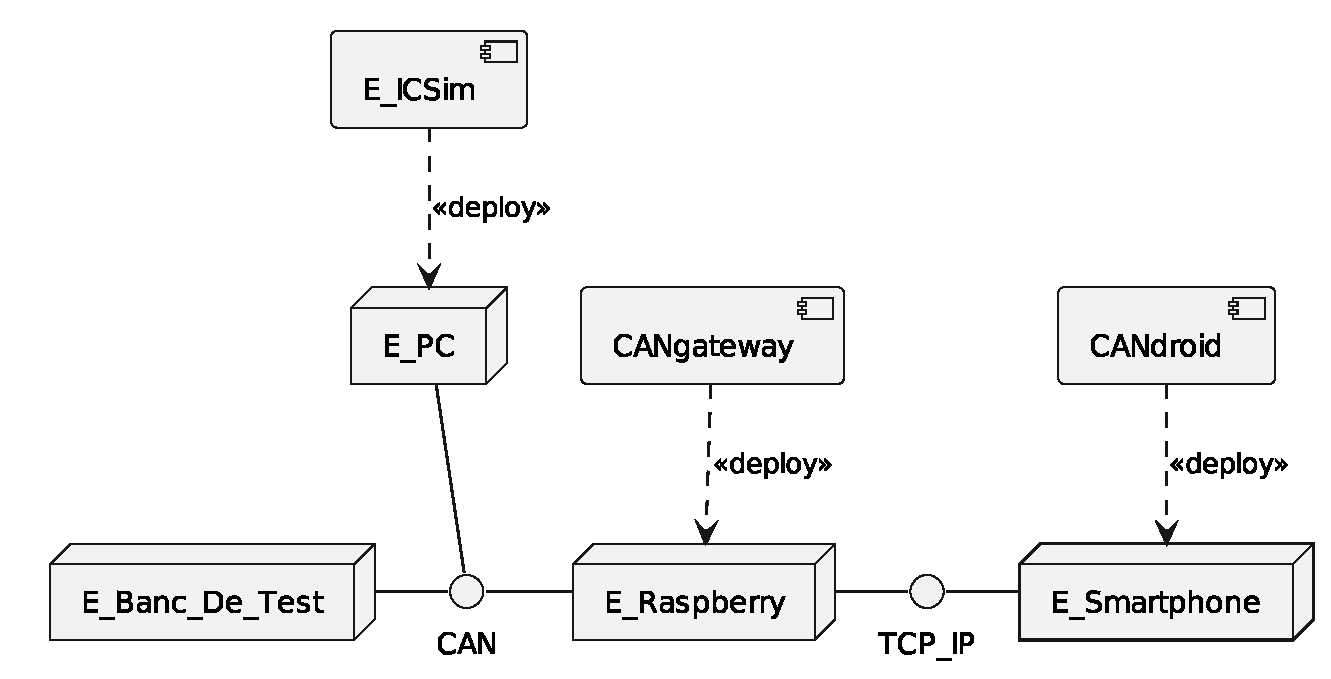
\includegraphics[width=14cm]{../schemas/arch_mat}
    \captionsetup{justification=centering}
    \caption{Architecture matérielle et logicielle représentée \\par un diagramme de déploiement UML}
    \label{schema_arch_mat}
\end{figure}

Comme indiqué sur le diagramme, l'application {\nomApplication} est déployée sur E\_Smartphone. Le programme {\nomLogiciel} est déployé sur E\_Raspberry. E\_Smartphone et E\_Raspberry communiquent ensemble grâce au protocole \hyperref[tcp_ip]{TCP/IP}. E\_Raspberry récupère les trames CAN émisent par E\_PC et/ou E\_Banc\_De\_Test grâce au RS485 CAN Hat qui permet à E\_Raspberry d'utiliser le protocole de communication CAN (Voir section \ref{dictionnaire}). E\_ICSim est un logiciel de simulation déployé sur E\_PC. Il permettra aux futurs utilisateurs de se former aux protocoles de communication CAN sans avoir à utiliser un Banc de test encombrant. Par convention, le nom de ces entités est préfixé par les caractères {\guillemotleft} E\_ {\guillemotright} (E pour Extern). Les caractéristiques de ces entités sont décrites dans le dictionnaire du domaine (voir section \ref{dictionnaire}).
\begin{figure}[ht] 
    \centering
    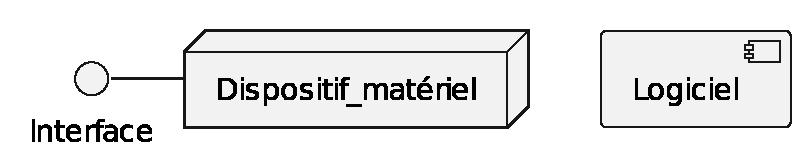
\includegraphics[width=10cm]{../schemas/legende_diag_deploiement}
    \caption{Légende du diagramme de déploiement UML}
    \label{schema_legende_diag_deploiment}
\end{figure}

\bigskip

% TODO relire et modifier les warnings
\newpage
\subsubsection{Les interfaces du système}
Cette section décrit les entrées et sorties dites « logiques » et « physiques » du SàE.
En effet, nous différencions dans cette étude deux grands types d'entrées/sorties : 
\begin{itemize}
  \item Celles dites de haut niveau (dites aussi logiques) qui décrivent les données échangées et événements entre Utilisateur, le SàE et E\_TableauDeBord. Les entrées/sorties logiques seront décrites à la section \ref{interfaces_logiques}.
  \item Celles dites de bas niveau (dites aussi physiques) qui sont les entrées/sorties réellement échangées entre le SàE et E\_TableauDeBord. Les entrées/sorties physiques 
  (ou bas niveau) seront décrites au chapitre \ref{interfaces_physiques}.
\end{itemize}

\paragraph{Les interfaces logiques}
\label{interfaces_logiques}
Le SàE est constitué d'une application Android nommée {\nomApplication} et un programme embarqué sur la Raspberry Pi nommé {\nomLogiciel}. 

\vspace{6pt}

La figure \ref{schema_contexte_log} présente le contexte en faisant figurer les entrées/sorties logiques. Cette représentation du contexte est sous la forme d'un diagramme de communication UML. Les éléments soulignés correspondent à des ensembles de messages qui vont être détaillés. \\

\begin{figure}[ht] 
    \centering
    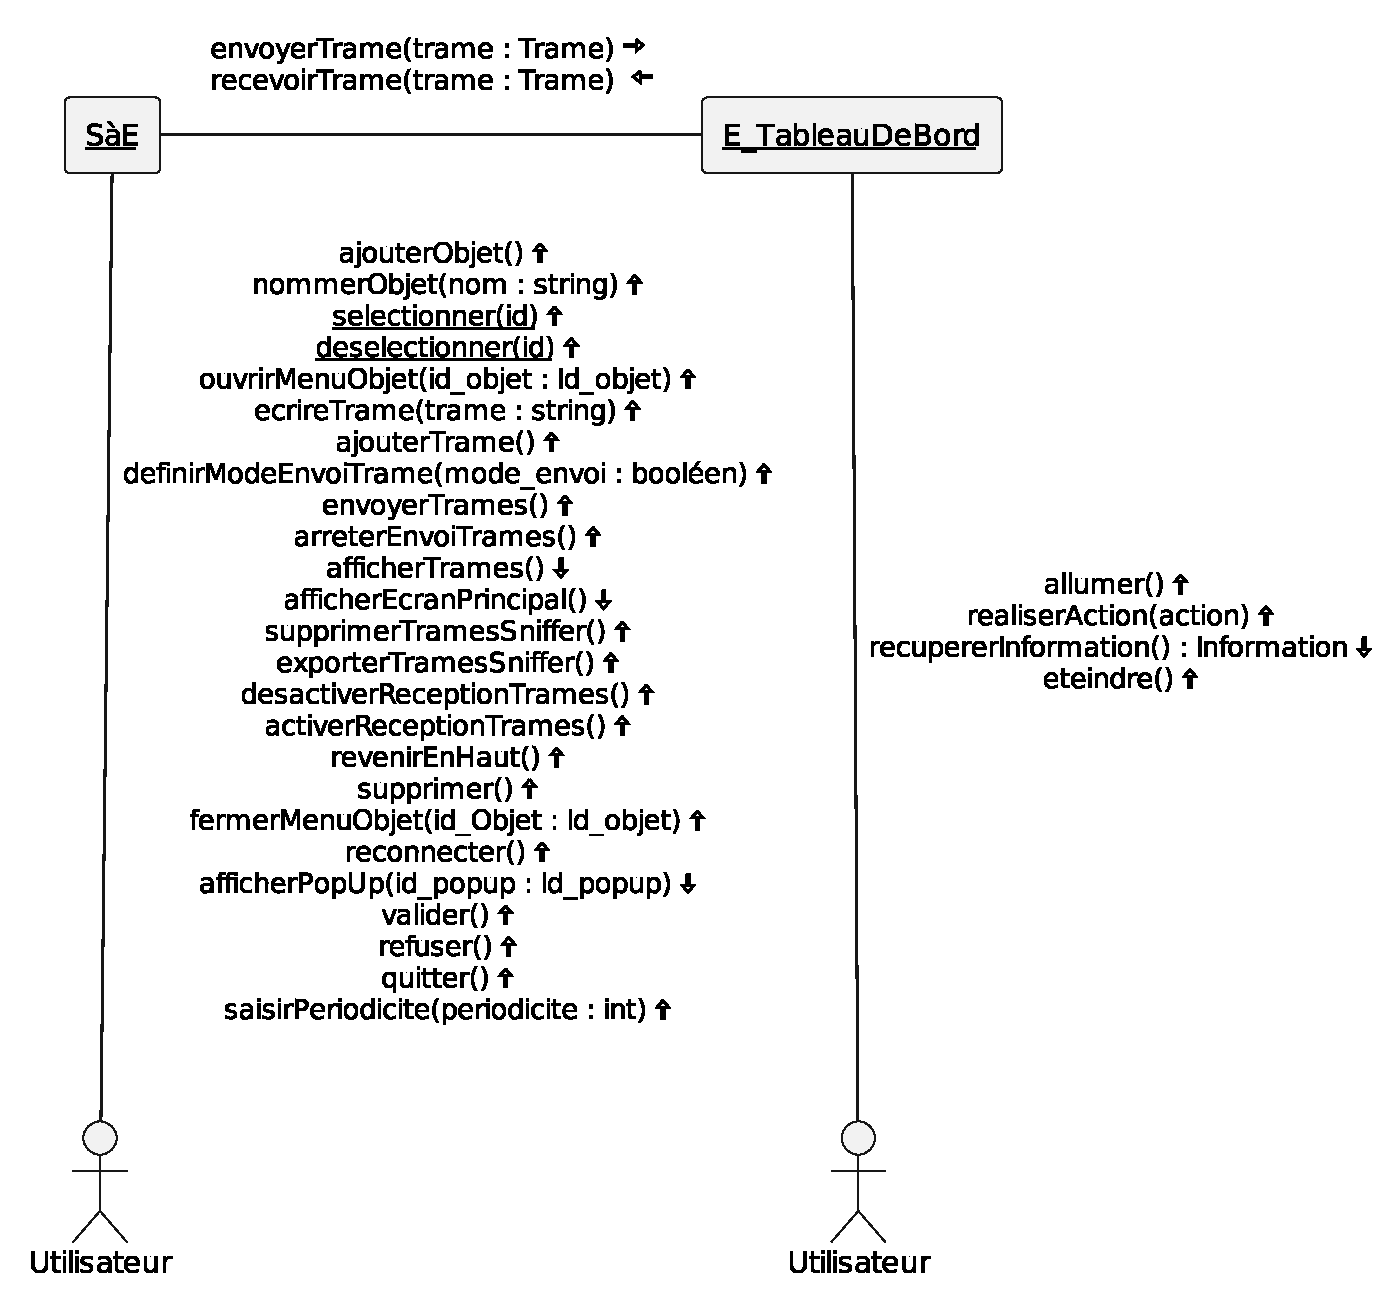
\includegraphics[width=12cm]{../schemas/contexte_log}
    \caption{Contexte logique représenté par un\\diagramme de communication UML}
    \label{schema_contexte_log}
\end{figure}

\newpage

\paragraph{Les interfaces avec les acteurs} 
L'acteur Utilisateur est en contact direct avec le SàE et Tableau de Bord. Les entrées et sorties entre Utilisateur et le SàE font référence aux fonctionnalités présentes sur l'IHM. Ces fonctionnalités sont décrites en détails dans la partie Exigences spécifiques (cf. section \ref{exigences_specifiques}). \\

Les listes d'objets et de trames mentionnées dans les descriptions suivantes sont initialement vides lors du premier lancement de l'application, mais elles sont affichées sur l'IHM. Nous allons maintenant détailler ces entrées et sorties logiques.

\vspace{-1cm}
\subparagraph{En provenance de Utilisateur}
\vspace{1cm}
\mbox{}\\

\textbf{Vers le SàE :} \vspace{0.2cm}\\ %SUBSUBPARAGRAPHE ?
\textbf{ajouterObjet()} --- Utilisateur ajoute un nouvel objet, un pop-up s'affiche ensuite pour nommer l'objet et valider l'ajout. \\
\textbf{nommerObjet(nom : string) } --- Utilisateur nomme l'objet créé dans le pop-up qui s'est affiché. Une validation est attendue. \\
\textbf{ \underline{selectionner(id)}} : 
\begin{itemize}
    \item \textbf{selectionnerObjet(id\_objet : Id\_objet)} --- Utilisateur sélectionne un objet d'ID id\_objet, il se grise ensuite. 
    \item \textbf{selectionnerTrame(id\_trame : Id\_trame)} --- Utilisateur sélectionne une trame d'ID id\_trame, elle se grise ensuite. 
\end{itemize}
\textbf{ \underline{deselectionner(id)}} : 
\begin{itemize}
    \item \textbf{deselectionnerObjet(id\_objet : Id\_objet)} --- Utilisateur désélectionne un objet d'ID id\_objet, il se dégrise ensuite. 
    \item \textbf{deselectionnerTrame(id\_trame : Id\_trame)} --- Utilisateur désélectionne une trame d'ID id\_trame, elle se dégrise ensuite. Lorsqu'il quitte le {\guillemotleft} Mode Envoi {\guillemotright}, les trames se désélectionnent automatiquement. 
\end{itemize}
\textbf{ouvrirMenuObjet(id\_objet : Id\_objet)} --- Utilisateur ouvre le menu déroulant d'un objet d'ID id\_objet. \\
\textbf{ecrireTrame(trame : string)} --- Utilisateur écrit une trame dans le menu déroulé d'un objet, le format de la trame est détaillé dans le dictionnaire de domaine (section \ref{dictionnaire}). \\
\textbf{ajouterTrame()} --- Utilisateur ajoute la trame écrite, un pop-up s'affiche pour définir le Mode Envoi de la trame.\\
\textbf{definirModeEnvoiTrame(mode\_envoi : booléen)} --- Utilisateur définit un Mode Envoi pour la trame à ajouter. Si vrai, l'envoi est ponctuel. Si faux, l'envoi est cyclique. Une validation est attendue. \\
\textbf{envoyerTrames()} --- Utilisateur demande à envoyer la ou les trames préalablement ajoutées(s) et sélectionnée(s). L'application {\nomApplication} passe alors en {\guillemotleft} Mode Envoi {\guillemotright}, et Utilisateur ne peut plus supprimer de trames ou ajouter d'objets. L'envoi des trames continue même si Utilisateur met en veille l'application {\nomApplication}.  \\
\textbf{arreterEnvoiTrames()} --- Utilisateur arrête l'envoi des trames. L'application {\nomApplication} quitte le {\guillemotleft} Mode Envoi {\guillemotright} et Utilisateur a de nouveau accès aux fonctionnalités de suppression d'élément et d'ajout d'objet.\\
\textbf{supprimerTramesSniffer()} --- Utilisateur supprime l'ensemble des trames affichées dans le sniffer. \\
\textbf{exporterTramesSniffer()} --- Utilisateur demande à exporter l'ensemble des trames affichées dans le sniffer dans un fichier de logs (voir section \ref{dictionnaire}). \\
\textbf{desactiverReceptionTrames()} --- Utilisateur désactive la réception de trames, le SàE ne va plus afficher les trames en provenance de Tableau de Bord sur l'IHM. \\
\textbf{activerReceptionTrames()} --- Utilisateur demande à activer la réception des trames, L'application {\nomApplication} affiche les trames en provenance de Tableau de Bord sur l'IHM. La reception des trames continue même si Utilisateur met en veille l'application {\nomApplication}. \\
\textbf{revenirEnHaut()} --- Utilisateur revient en haut du fil de trames affichées dans le sniffer. \\
\textbf{supprimer()} --- Utilisateur supprime les trames et objets sélectionnés. Si Utilisateur a sélectionné un ou plusieurs objets, les trames ajoutées dans le menu de ces objets seront aussi supprimées. \\
Un pop-up s'affiche pour confirmer ou non la suppression. \\
\textbf{fermerMenuObjet(id\_objet : Id\_objet)} --- Utilisateur ferme le menu précédemment ouvert d'un objet d'ID id\_objet. \\
\textbf{reconnecter()} --- Utilisateur demande à reconnecter l'application {\nomApplication} au programme {\nomLogiciel}, un pop-up s'affiche et une validation est demandée. \\
\textbf{valider()} --- Utilisateur choisit de valider son action lorsque qu'un pop-up s'affiche. \\
\textbf{refuser()} --- Utilisateur choisit de refuser de réaliser son action lorsque qu'un pop-up s'affiche.\\
\textbf{quitter()} --- Utilisateur quitte l'application {\nomApplication}. \\
\textbf{saisirPeriodicite(periodicite : int)} --- Utilisateur saisit la périodicité de la trame qu'il veut envoyer en mode cyclique. \\
\textbf{demarrer\_SSH()} --- Utilisateur démarre le programme {\nomApplication}. Le démarrage s'effectue en ligne de commande via une connexionn SSH à la Raspberry Pi. \\
\textbf{quitter\_SSH()} --- Utilisateur quitte le programme {\nomApplication}. L'arrêt s'effectue en ligne de commande via une connexionn SSH à la Raspberry Pi. \\


\textbf{Vers E\_TableauDeBord :} \vspace{0.2cm} \\ %SUBSUBPARAGRAPHE !
Les fonctions décrites ci-dessous s'exécutent en arrière-plan. \\
\\
\textbf{allumer()} --- Utilisateur allume Tableau de Bord. \\
\textbf{realiserAction(action)} --- Utilisateur réalise une action sur Tableau de Bord. \\
\textbf{recupererInformation() : Information} --- Utilisateur récupère des informations sur Tableau de Bord grâce aux indicateurs visuels. \\
\textbf{eteindre()} --- Utilisateur éteint Tableau de Bord.

\subparagraph{En provenance du SàE}
\mbox{}\\\\
\textbf{Vers Utilisateur :} \vspace{0.2cm} \\ %SUBSUBPARAGRAPHE !
\textbf{afficherEcranPrincipal()} --- L'application {\nomApplication} affiche l'écran principal. \\
\textbf{afficherTrames()} --- L'application {\nomApplication} affiche toutes les trames du sniffer, c'est-à-dire les trames qu'il a sniffées en provenance de Tableau de Bord, et les trames que Utilisateur a envoyées.  \\
\textbf{afficherPopUp(id\_popup : Id\_popup)} --- L'application {\nomApplication} affiche un pop-up d'ID id\_popup correspondant à l'action réalisée précédemment par Utilisateur (voir section \ref{dictionnaire}). \\

\textbf{Vers E\_TableauDeBord :} \vspace{0.2cm} \\ %SUBSUBPARAGRAPHE !
\textbf{envoyerTrame(trame : Trame)} --- Le SàE transmet à Tableau de Bord les trames que Utilisateur a décidé d'envoyer (voir section \ref{dictionnaire} pour les détails sur le type Trame).
\subparagraph{En provenance de E\_TableauDeBord}
\mbox{}\\

\textbf{Vers le SàE :} \vspace{0.2cm} \\ %SUBSUBPARAGRAPHE !
\textbf{recevoirTrame(trame : Trame)} --- Le SàE reçoit des trames envoyées par Tableau de Bord (voir section \ref{dictionnaire} pour les détails sur le type Trame).

\paragraph{Les interfaces physiques}
\label{interfaces_physiques}
Ce paragraphe précise les caractéristiques de chaque interface entre le logiciel et les composants matériels du
système. Il s'agit des entrées/sorties physiques. Ce sont celles que devra réellement traiter le SàE 
en les interprétant ou les générant en événement logiques. \\

La figure \ref{schema_contexte_phy} représente ce contexte physique avec un diagramme de communication UML.

\begin{figure}[ht] 
    \centering
    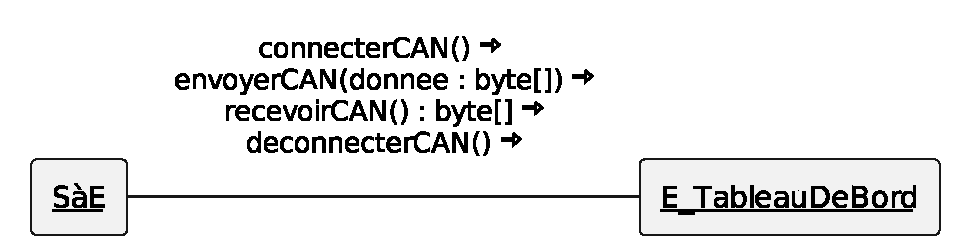
\includegraphics[width=14cm]{../schemas/contexte_phy}
    % \captionsetup{justification=centering}
    \caption{Contexte physique représenté \\par un diagramme de déploiement UML}
    \label{schema_contexte_phy}
\end{figure}

\subparagraph{En provenance du SàE}
\mbox{}\\

\textbf{Vers E\_TableauDeBord :} \vspace{0.2cm} \\ %SUBSUBPARAGRAPHE !
\textbf{connecterCAN()} --- Le SàE se connecte au bus CAN. \\
\textbf{envoyerCAN(donnee : byte[])} --- Le SàE envoie une ou plusieurs trames sur le bus CAN. \\
\textbf{recevoirCAN() : byte[] }--- Le SàE récupère la ou les trames sortantes de Tableau de Bord sur le bus CAN.  \\
\textbf{deconnecterCAN()} --- Le SàE se déconnecte du bus CAN. \\



% --------------------------
% CAS D'USAGE {p.12}
% --------------------------
%TODO
\newpage
\subsection{Fonctions principales développées}
Ce chapitre présente les principales fonctionnalités développées dans l'incrément 1 et 2 en utilisant une approche basée sur les cas d'usage et les cas d'utilisation (CU). Il met en évidence les fonctionnalités clés implémentées dans ces deux incréments, en les reliant aux cas d'usage et aux cas d'utilisation pertinents. 

\subsubsection{Rappel sur les cas d'usage}
Les cas d'usage recensent les étapes essentielles du cycle de vie d'un produit depuis la fabrication du produit jusqu'à l'élimination ou le recyclage du produit. \`A chaque étape du cycle de vie correspond un cas d'usage (si cette étape induit des fonctionnalités à définir pour le produit considéré). Pour chaque cas d'usage, plusieurs cas d'utilisation distincts peuvent être définis.\\
\newline
Parmi les cas d'usage, on retrouve généralement ceux de fabrication du produit (comprenant ou non les activités de test du produit fabriqué), de conditionnement (paramétrage éventuel, expédition et transport), de commercialisation (paramétrage éventuel, mode de démonstration, installation sur site...), d'utilisation (par le ou les utilisateurs), de maintenance (SAV ou diagnostique), de désinstallation et de recyclage (élimination ou valorisation).
\medskip

\subsubsection{Rappel sur les cas d'utilisation}
\medskip
Un cas d'utilisation (CU) représente un ensemble d'interactions entre un ou des acteurs et le système à spécifier. Ce cas d'utilisation est souvent lié à un ou parfois plusieurs cas d'usage. Un CU est principalement décrit par un scénario d'utilisation (nommé scénario nominal), scénario d'une utilisation représentative du système. Ces CU sont ensuite détaillés jusqu'à un niveau de décomposition suffisant pour décrire les fonctions attendues du système. 
\medskip

\paragraph{Représentation graphique des CU}
%~\par
Les CU peuvent être représentés sous forme graphique, voir la figure \ref{schema_diag_cu} pour un exemple. Les acteurs directs sont représentés sous forme de petits personnages. Dans les bulles, sont représentés les cas d'utilisation. Un trait entre un acteur et un CU indique que l'acteur participe à ce CU. Les liens hachurés entre CU, étiquetés par le mot <<use>> (ou <<include>>), indiquent que ce CU fait appel à l'autre CU --- on parle alors de sous-cas d'utilisation. Les liens hachurés entre CU, étiquetés par le mot <<extend>>, indique qu'il s'agit d'une extension d'un CU : un CU qui ne se déclenche que sous certaines conditions.

\begin{minipage}{1\linewidth} 
    \centering
    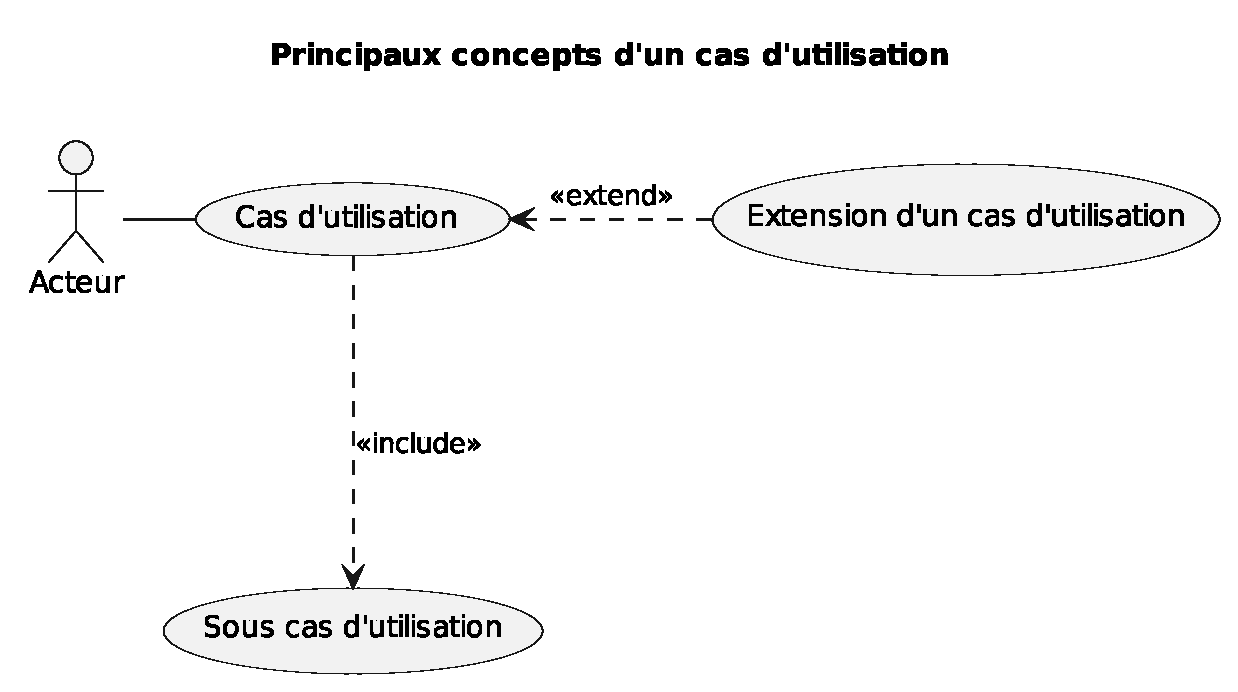
\includegraphics[width=14cm]{../schemas/exemple_diag_cu}
    \captionsetup{justification=centering}
    \captionof{figure}{Légende explicative d'un diagamme de cas d'utilisation UML}
    \label{schema_diag_cu}
\end{minipage}

\paragraph{Représentation textuelle des CU}
%~\par
La description textuelle des cas d'utilisation est souvent présentée sous forme d'un tableau constitué de champs suivants : 
\begin{longtable}[l]{|p{3cm}|p{11.7cm}|}
    \hline
        Titre & Rappelle en quelques mots l'objectif principal du cas d'utilisation.\\
    \hline
        Résumé & Décrit brièvement le comportement du cas d'utilisation.\\
    \hline
        Portée & Définit la portée de conception du CU (étendue spatiale).\\
    \hline
        Niveau & Niveau de granularité du cas d'utilisation (stratégique, utilisateur ou sous-fonction).\\
    \hline
        Acteurs directs & Acteurs qui participent au CU.\\
    \hline 
        Acteurs indirects & Acteurs qui ne participent pas au CU, mais qui ont un intérêt dans sa réalisation.\\
    \hline
        Préconditions & Ensemble des conditions qui doivent être vérifiées avant le déroulement du CU. Les
        préconditions, sans mention contraire explicite, des CU parents au CU doivent
        toujours être vérifiées.\\
    \hline
        Garanties \newline minimales & Définissent ce qui est garanti par le système à l'étude même en cas d'échec du cas d'utilisation.\\
    \hline
        Garanties en cas de succès & Définissent les garanties en cas de succès (par le scénario nominal ou par ses
        variantes). \\
    \hline
        Scénario nominal & C'est un scénario représentatif de l'utilisation du système où tout se passe bien. Il
        se termine par la réussite des objectifs. Il peut être constitué d'une condition
        déclenchant le scénario, d'un ensemble d'étapes, d'une condition de fin, et
        éventuellement d'extensions ou de variantes. Une étape peut être une interaction
        entre acteurs, une étape de validation, ou un changement interne.\\
    \hline
        Variantes & Lorsqu'il y a plusieurs façons de procéder à une même étape sans remise en cause
        du scénario nominal.\\
    \hline
        Extensions & Définissent les autres scénarios que le scénario nominal (par exemple ceux qui se
        terminent par un échec). Ils se déclenchent sur des conditions spécifiques
        détectées par le SàE.\\
    \hline
        Informations \newline complémentaires & Informations diverses nécessaires à la compréhension du CU. \\
    \hline
\end{longtable}

% ----------------------------------------------
% CU STRATEGIQUE
% ----------------------------------------------
\newpage
\subsubsection{CU Échanger des trames CAN}
\paragraph{Description graphique}
\medskip
\begin{minipage}{1\linewidth}
    \centering
    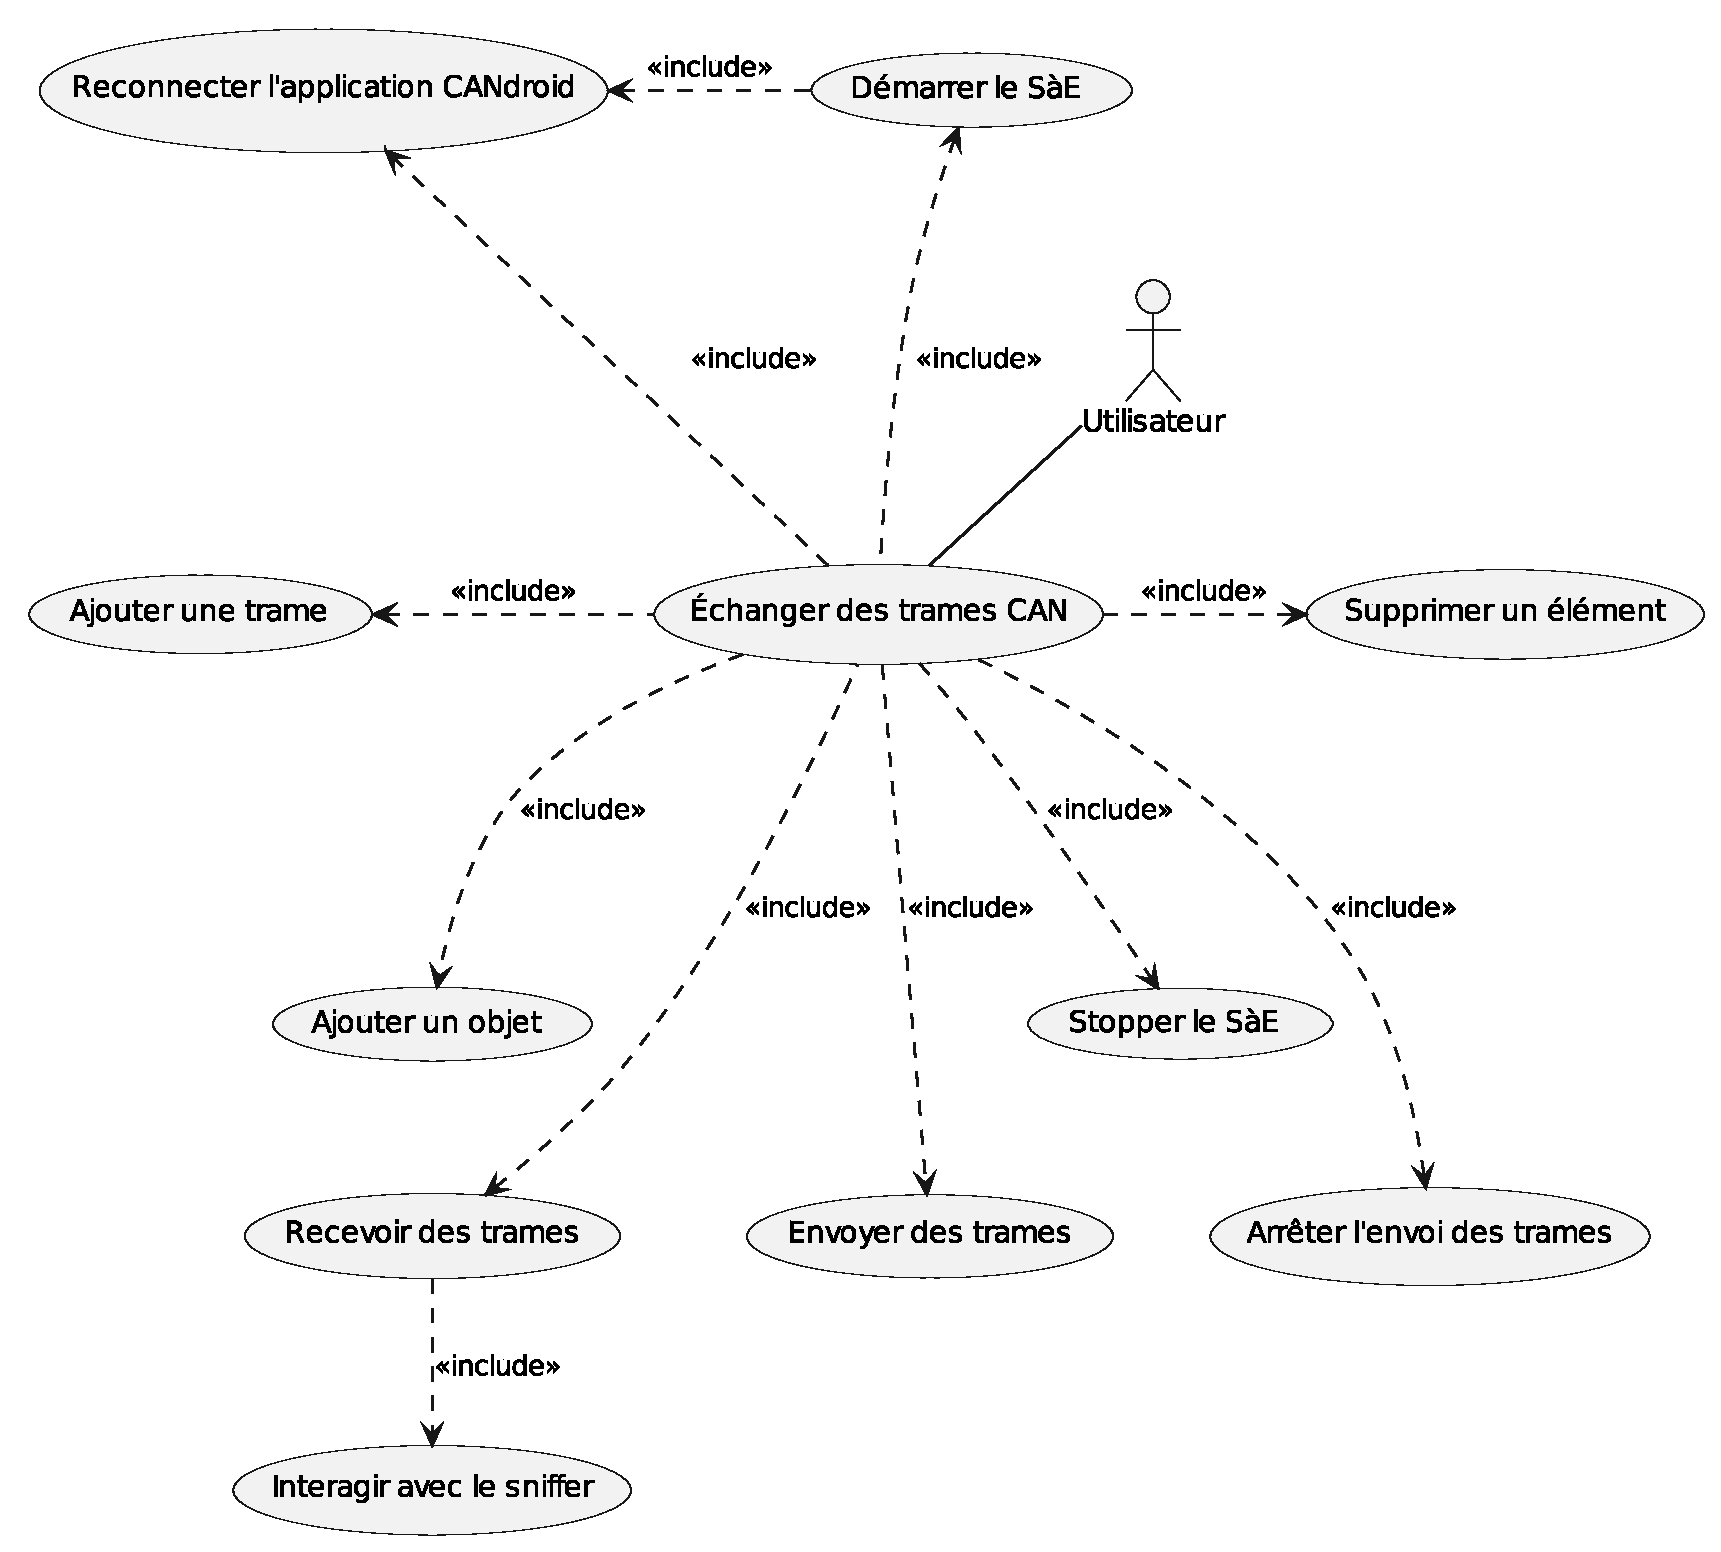
\includegraphics[width=15cm]{../../specification/schemas/cu_strat}
    \captionof{figure}{CU Échanger des trames CAN}
    \label{schema_cu_strat}
\end{minipage}

\newpage
\paragraph{Description textuelle}
\medskip

\begin{longtable}[l]{|p{3cm}|p{11.7cm}|}
    \hline
    
        Titre & Échanger des trames CAN.\\
    \hline
    
        Résumé & Utilisateur peut échanger des trames CAN avec Tableau de Bord. \\
    \hline
    
        Portée & SàE.\\
    \hline
    
        Niveau & Stratégique.\\
    \hline
    
        Acteurs directs & Utilisateur.\\
    \hline 
    
        Acteurs indirects & N.A. \\
    \hline
    
    Préconditions & 
        \begin{itemize}
            \item Tableau de Bord et la Raspberry Pi sont fonctionnels.
            \item Le programme {\nomLogiciel} est installé sur la Raspberry Pi.
            \item L'application {\nomApplication} est téléchargée sur le Smartphone.
            \item Le matériel est fonctionnel.
        \end{itemize} \\
    \hline
    
    Garanties \newline minimales & 
    \begin{itemize}
        \item L'application {\nomApplication} est utilisable.
    \end{itemize}
         \\
    \hline
    
    Garanties en cas de succès & 
    \begin{itemize}
        \item Utilisateur peut échanger des trames CAN entre Tableau de Bord et l'application {\nomApplication}.
        \item Utilisateur est capable d'observer les trames CAN reçues et d'en envoyer des nouvelles.
        \item Utilisateur est capable d'ajouter des objets ainsi que d'ajouter des trames à envoyer.
    \end{itemize}
         \\
    \hline
    
    Scénario nominal &
    \begin{enumerate}
        \item Utilisateur \underline{démarre le SàE}.
        \item Le SàE commence à \underline{recevoir des trames}.
        \item Utilisateur demande à \underline{ajouter un objet}.
        \item Utilisateur demande à \underline{ajouter une trame}.
        \item Utilisateur demande à \underline{envoyer des trames}.
        \item Le SàE diffuse les trames sur le bus CAN.
        \item Utilisateur demande à \underline{arrêter l'envoi des trames}.
        \item Utilisateur demande à \underline{supprimer un élément}.
        \item Utilisateur \underline{stoppe le SàE}.
    \end{enumerate} \\
    \hline

    Variantes & \newline
        \textbf{2,5 [La connexion n'est pas établie et Utilisateur ne souhaite pas se reconnecter]} \newline
            2,5.a.1. Va en 3. \newline
        \newline
        \textbf{2,5 [La connexion n'est pas établie \& Utilisateur souhaite se reconnecter]} \newline
            2,5.b.1. Utilisateur demande à \underline{reconnecter l'application {\nomApplication}} au programme {\nomLogiciel}. \newline
            2,5.b.2. Va en 2.\newline
        \newline
        \textbf{3,4,5,7,8 [Utilisateur souhaite stopper le SàE]}\newline
            3,4,5,7,8.a.1. Va en 9. \newline
        \newline
        \textbf{3,4,5,7,9 [Un élément existe \& Utilisateur souhaite supprimer un élément]}\newline
            3,4,5,7,9.a.1. Va en 8. \newline
        \newline
        \textbf{3,4,5,8,9 [Des trames sont en cours d'envoi \& Utilisateur souhaite arrêter l'envoi de trames]} \newline
        3,4,5,8,9.a.1. Va en 7. \newline
        \newline
        \textbf{3,4,7,8,9 [Au moins une trame existe, aucune trame n'est en cours d'envoi \& Utilisateur souhaite envoyer une trame]} \newline
        3,4,7,8,9.a.1. Va en 5. \newline
        \newline
        \textbf{3,5,7,8,9 [Utilisateur souhaite ajouter une trame \& au moins un objet existe]} \newline
        3,5,7,8,9.a.1. Va en 4. \newline
        \newline
        \textbf{4,5,7,8,9 [Utilisateur souhaite ajouter un objet]} \newline
            4,5,7,8,9.a.1. Va en 3. \newline
        \newline
        \textbf{5 [Il n'y a pas de trames à envoyer]} \newline
            5.a.1. Va en 8. \newline
        \newline
        \textbf{7 [Il n'y a pas de trames en cours d'envoi]} \newline
            7.a.1. Va en 8. \newline
        \newline
        \textbf{8 [Il n'y a pas d'éléments à supprimer]} \newline
            8.a.1. Va en 9. \newline
        \\
    \hline

    Extensions & \newline
        \textbf{2,6 [Utilisateur souhaite forcer l'arrêt du système]} \newline
        2,6.a.1. Va en 9. \newline
        \newline
        \\
    \hline
        Informations \newline complémentaires & N.A. \\
    \hline

\end{longtable}


\newpage

% ----------------------------------------------
% CU DEMARRER LE SAE
% ----------------------------------------------
\newpage
\subsubsection{CU Démarrer le SàE}
\paragraph{Description graphique}
Voir figure \ref{schema_cu_strat}.
\paragraph{Description textuelle}
\medskip

\begin{longtable}[l]{|p{3cm}|p{11.7cm}|}
    \hline
    
        Titre & Démarrer le SàE.\\
    \hline

        Résumé & Utilisateur démarre le SàE et les différents périphériques dont il a besoin. \\
    \hline

        Portée & SàE.\\
    \hline

        Niveau & Utilisateur.\\
    \hline

        Acteurs directs & Utilisateur.\\
    \hline 

        Acteurs indirects & N.A. \\
    \hline

        Préconditions & 
        \begin{itemize}
            \item Utilisateur à accès aux différents éléments du SàE ainsi que des différents périphériques dont il a besoin.
            \item Utilisateur est connecté à la Raspberry Pi en SSH.
        \end{itemize} \\ 
    \hline

        Garanties \newline minimales & N.A. \\
    \hline

        Garanties en cas de succès & 
        \begin{itemize}
            \item Utilisateur peut utiliser l'application {\nomApplication} librement. 
        \end{itemize}
        \\
    \hline
        Scénario nominal &
        \begin{enumerate}
            \item Utilisateur met en fonctionnement le Simulateur ICSim. 
            \item Utilisateur connecte la Raspberry Pi au bus CAN.
            \item Utilisateur met sous tension la Raspberry Pi.
            \item Utilisateur lance le programme {\nomLogiciel} via la \newline connexion SSH.
            \item E\_PC informe Utilisateur que le programme \newline {\nomLogiciel} est lancé.
            \item Utilisateur connecte E\_Smartphone au réseau TCP/IP de E\_Raspberry.
            \item E\_Smartphone informe Utilisateur qu'il est connecté au réseau TCP/IP de E\_Raspberry.
            \item Utilisateur démarre l'application {\nomApplication}.
            \item L'application {\nomApplication} affiche EcranPrincipal.
            \item L'application {\nomApplication} se connecte au programme \newline {\nomLogiciel}.
            \item L'application {\nomApplication} met à jour EcranPrincipal.
        \end{enumerate} \\
    \hline

    Variantes &     \newline
        \textbf{1 [Mise en fonctionnement du Banc de test uniquement]} \newline
        1.a.1. Utilisateur allume le Banc de test. \newline
        1.a.2. Va en 2. \newline
        \newline
        \textbf{1 [Mise en fonctionnement du Simulateur ICSim et du Banc de test]} \newline
        1.b.1. Utilisateur allume le Simulateur ICSim. \newline
        1.b.2. Utilisateur allume le Banc de test. \newline
        1.b.3. Va en 2. \newline
        \newline
        \textbf{1 [Utilisateur ne souhaite pas utiliser Tableau de Bord]} \newline
        1.c.1. Va en 2. \newline
        \newline
        \textbf{1-3 [Utilisateur ne souhaite pas utiliser la Raspberry Pi]} \newline
        1-3.a.1. Va en 8. \newline
        \newline
        \textbf{5 [Le programme {\nomLogiciel} ne s'est pas lancé]}\newline
        5.a.1 Utilisateur démarre l’application {\nomApplication}.\newline
        5.a.2 L’application {\nomApplication} affiche EcranPrincipal.\newline
        5.a.3 Fin du CU. \newline
        \newline
        \textbf{7 [La connexion échoue \& Utilisateur ne souhaite pas se reconnecter]} \newline
        7.a.1. Va en 8. \newline
        \newline
        \textbf{7 [La connexion échoue \& Utilisateur souhaite se reconnecter]}\newline
        7.b.1 Va en 6. \newline
        \newline
        \textbf{10 [La connexion échoue \& Utilisateur ne souhaite pas se reconnecter]} \newline
        10.a.1. Fin du CU. \newline
        \newline
        \textbf{10 [La connexion échoue \& Utilisateur souhaite se reconnecter]} \newline
        10.b.1. Utilisateur demande à \underline{reconnecter l'application {\nomApplication}} au programme {\nomLogiciel}. \newline
        10.b.2. Fin du CU. \newline
        \\
    \hline
    Extensions & N.A. \\
    \hline
    Informations \newline complémentaires & N.A. \\
    \hline
\end{longtable}

% ----------------------------------------------
% CU DEMARRER LE SAE
% ----------------------------------------------
\newpage
\subsubsection{CU Reconnecter l'application {\nomApplication}}
\paragraph{Description graphique}
\medskip
Voir figure \ref{schema_cu_strat}.
\paragraph{Description textuelle}
\medskip

\begin{longtable}[l]{|p{3cm}|p{11.7cm}|}
    \hline
    
        Titre & Reconnecter l'application {\nomApplication}.\\
    \hline

        Résumé & Utilisateur peut reconnecter l'application {\nomApplication} au programme {\nomLogiciel}. \\
    \hline

        Portée & Application {\nomApplication}.\\
    \hline

        Niveau & Utilisateur.\\
    \hline

        Acteurs directs & Utilisateur.\\
    \hline 

        Acteurs indirects & N.A. \\
    \hline

        Préconditions & 
        \begin{itemize}
            \item L'application {\nomApplication} est déconnectée du programme \newline {\nomLogiciel}. 
        \end{itemize}
        \\
    \hline

        Garanties \newline minimales & N.A. \\
    \hline

        Garanties en cas de succès & 
        \begin{itemize}
            \item L'application {\nomApplication} est de nouveau connectée au programme {\nomLogiciel}.
            \item Utilisateur peut utiliser l’application {\nomApplication} librement.
        \end{itemize}
         \\
    \hline
        Scénario nominal &
        \begin{enumerate}
            \item Utilisateur demande la reconnexion de l'application \newline{\nomApplication} au programme {\nomLogiciel}. 
            \item L'application {\nomApplication} affiche PopupDemandeReconnexion.
            \item Utilisateur valide la reconnexion.
            \item L'application {\nomApplication} affiche EcranPrincipal.
            \item L'application {\nomApplication} se reconnecte au programme \newline {\nomLogiciel}.
            \item L'application {\nomApplication} met à jour EcranPrincipal.
        \end{enumerate} \\
    \hline

    Variantes &     \newline
        \textbf{3 [Utilisateur souhaite abandonner la reconnexion]} \newline
        3.a.1. Utilisateur annule la reconnexion. \newline
        3.a.2. L'application {\nomApplication} affiche EcranPrincipal. \newline
        3.a.3. Fin du CU.\newline
        \newline
        \textbf{5 [La connexion échoue \& Utilisateur ne souhaite pas se reconnecter]} \newline
        5.a.1. Fin du CU. \newline
        \newline
        \textbf{5 [La connexion échoue \& Utilisateur souhaite se reconnecter]} \newline
        5.b.1. Va en 1. \newline
        \\
    \hline

        Extensions & N.A. \\
    \hline
    Informations \newline complémentaires & N.A. \\
    \hline
\end{longtable}

% ----------------------------------------------
% CU Recevoir des trames
% ----------------------------------------------
\newpage
\subsubsection{CU Recevoir des trames}
\paragraph{Description graphique}
Voir figure \ref{schema_cu_strat}.
\medskip
\paragraph{Description textuelle}
\medskip

\begin{longtable}[l]{|p{3cm}|p{11.7cm}|}
    \hline
    
        Titre & Recevoir des trames.\\
    \hline

        Résumé & L'application {\nomApplication} reçoit et affiche les trames du réseau CAN. \\
    \hline

        Portée & Application {\nomApplication}.\\
    \hline

        Niveau & Utilisateur.\\
    \hline

        Acteurs directs & Utilisateur.\\
    \hline 

        Acteurs indirects & N.A. \\
    \hline

        Préconditions & 
            \begin{itemize}
                \item Le SàE est démarré. 
                \item L'application {\nomApplication} est connectée au programme \newline {\nomLogiciel}.
                \item La Raspberry Pi est connectée au bus CAN.
                \item Tableau de Bord est connecté au bus CAN.
            \end{itemize}\\
    \hline

        Garanties \newline minimales & N.A. \\
    \hline

        Garanties en cas de succès & 
        \begin{itemize}
            \item Les trames sont affichées sur le sniffer de l'application \newline {\nomApplication}.
        \end{itemize}
        \\
    \hline

        Scénario nominal &
        \begin{enumerate}
            \item Utilisateur commande un actionneur sur Tableau de Bord.
            \item Le SàE récupère les trames du réseau CAN.
            \item L'application {\nomApplication} met à jour EcranPrincipal.
            \item Utilisateur demande à \underline{interagir avec le sniffer}.
        \end{enumerate} \\
    \hline

        Variantes & \newline
            \textbf{1-2 [La connexion échoue \& Utilisateur ne souhaite pas se reconnecter]} \newline
            1-2.a.1. Va en 3. \newline
            \newline
            \textbf{1-2 [La connexion échoue \& Utilisateur souhaite se reconnecter]} \newline
            1-2.b.1. Utilisateur demande à \underline{reconnecter l'application {\nomApplication}} au programme {\nomLogiciel}. \newline
            1-2.b.2. Va en 1. \newline
            \newline
            \textbf{4 [Utilisateur souhaite commander un autre actionneur]}\newline
            4.a.1. Va en 1. \newline
            \\
    \hline

        Extensions & \newline
        \textbf{2-3 [Utilisateur a demandé l'arrêt de la réception de trames]}
        2-3.a.1. Fin du CU. \newline
        \\
    \hline
    Informations \newline complémentaires & N.A. \\
    \hline
\end{longtable}

% ----------------------------------------------
% CU Interagir avec le sniffer
% ----------------------------------------------
\newpage
\subsubsection{CU Interagir avec le sniffer}
\paragraph{Description graphique}
Voir figure \ref{schema_cu_strat}.
\paragraph{Description textuelle}
\medskip

\begin{longtable}[l]{|p{3cm}|p{11.7cm}|}
    \hline
    
        Titre & Interagir avec le sniffer.\\
    \hline

        Résumé & Utilisateur interagit avec le sniffer. \\
    \hline

        Portée & Application {\nomApplication}.\\
    \hline

        Niveau & Utilisateur.\\
    \hline

        Acteurs directs & Utilisateur.\\
    \hline 

        Acteurs indirects & N.A. \\
    \hline

        Préconditions & 
            \begin{itemize}
                \item Le SàE est démarré. 
                \item L'application {\nomApplication} est connectée au programme \newline {\nomLogiciel}.
                \item La Raspberry Pi est connectée au bus CAN.
                \item Tableau de Bord est connecté au bus CAN.
            \end{itemize}\\
    \hline

        Garanties \newline minimales & N.A. \\
    \hline

        Garanties en cas de succès & 
        \begin{itemize}
            \item Utilisateur est capable d'exporter et de supprimer les trames du sniffer.
            \item Utilisateur est capable d'arrêter la mise à jour du sniffer en temps réel et de revenir en haut du fil lorsqu'il fait défiler les trames.
        \end{itemize}
        \\
    \hline

        Scénario nominal & 
        \begin{enumerate}
            \item Utilisateur demande de revenir en haut du fil.
            \item L'application {\nomApplication} va en haut du fil.
            \item Utilisateur demande d'effacer les trames.
            \item L'application {\nomApplication} efface les trames affichées.
            \item Utilisateur demande l'arrêt de la réception des trames.
            \item L'application {\nomApplication} stoppe l'affichage de nouvelles trames.
            \item Utilisateur demande d'enregistrer les trames reçues sur le \newline Smartphone.
            \item L'application {\nomApplication} enregistre les trames dans un fichier de log (voir section \ref{dictionnaire}).
            \item Utilisateur demande la reprise de la réception des trames.
            \item L'application {\nomApplication} reprend l'affichage de nouvelles trames.
        \end{enumerate} \\
    \hline

        Variantes & \newline
            \textbf{1,3,5,7 [La réception de trames est arrêtée \& Utilisateur souhaite reprendre la réception de trames]}\newline
                1,3,5,7.a.1. Va en 9. \newline
            \newline
            \textbf{1,3,5,7,9 [Utilisateur ne souhaite rien faire]}\newline
                1,3,5,7,9.a.1. Fin du CU. \newline
            \newline
            \textbf{1,3,9 [La réception de trames est arrêtée \& Utilisateur souhaite enregistrer les trames reçues]}\newline
                1,3,9.a.1. Va en 7. \newline
            \newline
            \textbf{1,3,9 [La réception de trames est en cours \& Utilisateur souhaite arrêter la réception de trames]}\newline
                1,3,9.b.1. Va en 5. \newline
            \newline
            \textbf{1,3,9 [La réception de trames est en cours \& Utilisateur souhaite enregistrer les trames reçues]}\newline
                1,3,9.c.1. Va en 5. \newline
            \newline
            \textbf{1,5,7,9 [Utilisateur souhaite effacer les trames]}\newline
                1,5,7,9.a.1. Va en 3. \newline
            \newline
            \textbf{3,5,7,9 [Utilisateur souhaite aller en haut du fil]}\newline
                3,5,7,9.a.1. Va en 1. \newline
            \\
    \hline

        Extensions & N.A. \\
    \hline
    Informations \newline complémentaires & N.A. \\
    \hline
\end{longtable}

% ----------------------------------------------
% CU CREER UN NOUVEL OBJET
% ----------------------------------------------
\newpage
\subsubsection{CU Ajouter un objet}
\paragraph{Description graphique}
Voir figure \ref{schema_cu_strat}.
\paragraph{Description textuelle}
\medskip

\begin{longtable}[l]{|p{3cm}|p{11.7cm}|}
    \hline
    
        Titre & Ajouter un objet.\\
    \hline

        Résumé & Utillisateur ajoute un objet sur l'application {\nomApplication}. \\
    \hline

        Portée & Application {\nomApplication}.\\
    \hline

        Niveau & Utilisateur. \\
    \hline

        Acteurs directs & Utilisateur.\\
    \hline 

        Acteurs indirects & N.A. \\
    \hline

        Préconditions & 
        \begin{itemize}
            \item L'application {\nomApplication} est démarrée.
        \end{itemize} \\
    \hline

        Garanties \newline minimales & N.A. \\
    \hline

        Garanties en cas de succès & 
        \begin{itemize}
            \item Un objet est ajouté. 
        \end{itemize}
        \\
    \hline

    Scénario nominal &
    \begin{enumerate} 
        \item Utilisateur demande l'ajout d'un objet. 
        \item Le SàE choisit un Nom d'objet par défaut.
        \item L'application {\nomApplication} affiche PopupAjoutObjet.
        \item Utilisateur saisit un nom d'objet.
        \item Utilisateur valide l'ajout.
        \item L'application {\nomApplication} met à jour EcranPrincipal.
    \end{enumerate} \\
    \hline

        Variantes & \newline
        \textbf{2 [Nombre maximal d'objets atteint \& Utilisateur souhaite ajouter un objet]} \newline
        2.a.1. L’application {\nomApplication} affiche PopupErreurNombreObjet. \newline 
        2.a.2. Utilisateur ferme PopupErreurNombreObjet. \newline
        2.a.3. L’application {\nomApplication} affiche EcranPrincipal. \newline
        2.a.4. Fin du CU. \newline
        \newline
        \textbf{4 [Utilisateur ne souhaite pas saisir de nom]} \newline
        4.a.1. Va en 5. \newline
        \newline
        \textbf{6 [Utilisateur souhaite saisir un nom qui existe déjà]} \newline
        6.a.1. L'application {\nomApplication} affiche PopupErreurAjoutObjet. \newline
        6.a.2. Va en 4. \newline
        \\
    \hline

        Extensions & \newline
        \textbf{4-5 [Utilisateur souhaite annuler]} \newline
        4-5.a.1. Utilisateur ferme PopupAjoutObjet. \newline
        4-5.a.2. L’application {\nomApplication} affiche EcranPrincipal. \newline
        4-5.a.3. Fin du CU. \newline
        \\
    \hline
    Informations \newline complémentaires & N.A. \\
    \hline
\end{longtable}

% ----------------------------------------------
% CU Enregistrer des trames CAN
% ----------------------------------------------
\newpage
\subsubsection{CU Ajouter une trame}
\paragraph{Description graphique}
Voir figure \ref{schema_cu_strat}.
\paragraph{Description textuelle}
\medskip

\begin{longtable}[l]{|p{3cm}|p{11.7cm}|}
    \hline
    
        Titre & Ajouter une trame.\\
    \hline

        Résumé & Utilisateur ajoute une trame CAN associée à un objet avec son Mode Envoi. \\
    \hline

        Portée & Application {\nomApplication}.\\
    \hline

        Niveau & Utilisateur.\\
    \hline

        Acteurs directs & Utilisateur.\\
    \hline 

        Acteurs indirects & N.A. \\
    \hline

        Préconditions & 
        \begin{itemize}
            \item Le SàE est démarré.
            \item Un objet existe.
        \end{itemize} \\
    \hline

        Garanties \newline minimales & N.A.\\
    \hline

        Garanties en cas de succès & 
        \begin{itemize}
            \item Une trame est créée dans le bon objet.
        \end{itemize}
         \\
    \hline

        Scénario nominal &
        \begin{enumerate}
            \item Utilisateur déroule le menu de l'objet.
            \item L'application {\nomApplication} met à jour EcranPrincipal.
            \item Utilisateur saisit la trame. 
            \item Utilisateur valide la saisie de la trame.
            \item L'application {\nomApplication} affiche PopupModeEnvoiTrame.
            \item Utilisateur choisit le mode d'envoi ponctuel.
            \item Utilisateur valide le mode d'envoi.
            \item L'application {\nomApplication} affiche EcranPrincipal.
        \end{enumerate} \\
    \hline

        Variantes & \newline
        \textbf{1 [L’objet est déjà déplié]} \newline
            1.a.1. Va en 3.\newline
            \newline
        \textbf{5 [Nombre maximal de trames atteint \& Utilisateur souhaite
        ajouter une trame]} \newline
            5.a.1. L’application {\nomApplication} affiche PopupErreurNombreTrame.\newline
            5.a.2. Utilisateur ferme PopupErreurNombreTrame. \newline
            5.a.3. L’application {\nomApplication} affiche EcranPrincipal. \newline
            5.a.4. Fin du CU. \newline
            \newline
        \textbf{5 [Utilisateur souhaite ajouter une trame qui n'a pas le bon format]} \newline
            5.b.1. L'application {\nomApplication} affiche PopupErreurSaisieTrame. \newline
            5.b.2. Utilisateur ferme PopupErreurSaisieTrame. \newline
            5.b.3. L’application {\nomApplication} affiche EcranPrincipal. \newline
            5.b.4. Va en 3. \newline 
            \newline 
        \textbf{6 [Utilisateur choisit le mode cyclique \& souhaite changer la périodicité]} \newline
            6.a.1. Utilisateur choisit le mode d'envoi cyclique. \newline
            6.a.2. Utilisateur saisit la périodicité. \newline
            6.a.3. Va en 7. \newline
            \newline
        \textbf{6 [Utilisateur choisit le mode cyclique \& souhaite garder la périodicité par défaut]} \newline
            6.b.1. Utilisateur choisit le mode d'envoi cyclique. \newline    
            6.b.2. Va en 7. \newline
            \\
    \hline

        Extensions & \newline
        \textbf{6-7 [Utilisateur souhaite annuler]} \newline
        6-7.a.1. Utilisateur ferme PopupModeEnvoiTrame. \newline
        6-7.a.2. L'application {\nomApplication} affiche EcranPrincipal. \newline
        \\
    \hline
    Informations \newline complémentaires & N.A. \\
    \hline
\end{longtable}

% ----------------------------------------------
% CU ENVOYER DES TRAMES
% ----------------------------------------------
\newpage
\subsubsection{CU Envoyer des trames}
\paragraph{Description graphique}
Voir figure \ref{schema_cu_strat}.

\paragraph{Description textuelle}
\medskip

\begin{longtable}[l]{|p{3cm}|p{11.7cm}|}
    \hline
    
        Titre & Envoyer des trames.\\
    \hline
    
        Résumé & Utilisateur utilise l'application {\nomApplication} afin d'envoyer une trame CAN au Tableau de Bord. \\
    \hline
    
        Portée & SàE.\\
    \hline
    
        Niveau & Utilisateur\\
    \hline
    
        Acteurs directs & Utilisateur.\\
    \hline 
    
        Acteurs indirects & N.A. \\
    \hline
    
        Préconditions & 
        \begin{itemize}
            \item Le SàE est démarré.
            \item Un ou plusieurs objets existent.
            \item Une ou plusieurs trames existent.
            \item L'application {\nomApplication} est connectée au programme \newline {\nomLogiciel}.
            \item La Raspberry Pi est connectée au bus CAN.
            \item Tableau de Bord est connecté au bus CAN.
        \end{itemize}
        \\
    \hline
    
        Garanties \newline minimales & N.A. \\
    \hline
    
        Garanties en cas de succès & 
        \begin{itemize}
            \item La trame CAN est envoyée à Tableau de Bord.
        \end{itemize}
         \\
    \hline
    
        Scénario nominal & 
        \begin{enumerate}
            \item Utilisateur déroule le menu d'un objet.
            \item L'application {\nomApplication} met à jour EcranPrincipal.
            \item Utilisateur sélectionne une trame.
            \item L'application {\nomApplication} met à jour EcranPrincipal.
            \item Utilisateur demande à envoyer la trame.
            \item Le SàE diffuse la trame sur le bus CAN.
            \item L'application {\nomApplication} met à jour EcranPrincipal.
        \end{enumerate}
        \\
    \hline
        Variantes &     \newline
        \textbf{1 [L'objet est déjà déplié]} \newline
            1.a.1. Va en 3. \newline
            \newline
        \textbf{3 [Une trame est sélectionnée \& Utilisateur ne souhaite pas sélectionner de trames]} \newline
            3.a.1. Va en 5. \newline
            \newline
        \textbf{3 [Aucune trame n'est sélectionnée \& Utilisateur ne souhaite pas sélectionner de trames]} \newline
            3.b.1. Fin du CU. \newline
            \newline
        \textbf{5 [Utilisateur souhaite sélectionner plusieurs trames]} \newline
            5.a.1. Va en 1. \newline
            \newline
        \textbf{5 [Utilisateur ne souhaite plus envoyer de trames]} \newline
            5.b.1. Utilisateur désélectionne les trames grisées. \newline
            5.b.2. L'application {\nomApplication} met à jour EcranPrincipal. \newline
            5.b.3. Fin du CU. \newline
            \newline
        \textbf{5 [Utilisateur souhaite désélectionner une trame]}\newline
            5.c.1. Utilisateur désélectionne une trame grisée. \newline
            5.c.2. L'application {\nomApplication} met à jour EcranPrincipal. \newline
            5.c.3. Va en 3. \newline
            \newline
        \textbf{6 [Une ou plusieurs trames sélectionnées sont paramétrées avec le Mode Envoi cyclique]} \newline
            6.a.1. Le SàE commence l'envoi des trames sélectionnées sur le bus CAN. \newline
            6.a.2. Va en 7. \newline
        \\
    \hline
        Extensions &  N.A. \\
     
    \hline
    Informations \newline complémentaires & N.A. \\
    \hline
\end{longtable}

% ----------------------------------------------
% CU Arreter l'envoi des trames 
% ----------------------------------------------
\newpage
\subsubsection{CU Arrêter l'envoi des trames}
\paragraph{Description graphique}
Voir figure \ref{schema_cu_strat}.

\paragraph{Description textuelle}
\medskip

\begin{longtable}[l]{|p{3cm}|p{11.7cm}|}
    \hline
    
        Titre & Arrêter l'envoi des trames.\\
    \hline
    
        Résumé & Utilisateur utilise l'application {\nomApplication} afin d'arrêter l'envoi des trames à Tableau de Bord. \\
    \hline
    
        Portée & SàE.\\
    \hline
    
        Niveau & Utilisateur.\\
    \hline
    
        Acteurs directs & Utilisateur.\\
    \hline 
    
        Acteurs indirects & N.A. \\
    \hline
    
        Préconditions & 
        \begin{itemize}
            \item Le SàE est démarré.
            \item L'application {\nomApplication} est connectée au programme \newline {\nomLogiciel}.
            \item La Raspberry Pi est connectée au bus CAN.
            \item Tableau de Bord est connecté au bus CAN.
            \item Un ou plusieurs objets existent.
            \item Une ou plusieurs trames existent.
            \item Une ou plusieurs trames sont en cours d'envoi.
        \end{itemize}
        \\
    \hline
    
        Garanties \newline minimales & N.A. \\
    \hline
    
        Garanties en cas de succès & 
        \begin{itemize}
            \item Plus aucune trame CAN n'est envoyée à Tableau de Bord.
        \end{itemize}
         \\
    \hline
    
        Scénario nominal &
        \begin{enumerate}
            \item Utilisateur demande à stopper l'envoi des trames.
            \item L'application {\nomApplication} affiche PopupArretEnvoi.
            \item Utilisateur confirme l'arrêt de l'envoi des trames.
            \item Le SàE arrête de diffuser les trames sur le bus CAN.
            \item L'application {\nomApplication} affiche EcranPrincipal.
        \end{enumerate}
        \\
    \hline
        Variantes & \newline
        \textbf{3 [Utilisateur ne souhaite plus arrêter l'envoi des trames]} \newline
            3.a.1. Utilisateur ferme le pop-up. \newline
            3.a.2. Va en 5. \newline
        \\
    \hline
        Extensions &  N.A. \\
     
    \hline
    Informations \newline complémentaires & N.A. \\
    \hline
\end{longtable}

% ----------------------------------------------
% CU Supprimer un élement 
% ----------------------------------------------
\newpage
\subsubsection{CU Supprimer un élément}
\paragraph{Description graphique}
Voir figure \ref{schema_cu_strat}.

\paragraph{Description textuelle}
\medskip

\begin{longtable}[l]{|p{3cm}|p{11.7cm}|}
    \hline
    
        Titre & Supprimer un élément.\\
    \hline
    
        Résumé & Utilisateur utilise l'application {\nomApplication} pour supprimer une trame ou un objet. \\
    \hline
    
        Portée & SàE.\\
    \hline
    
        Niveau & Utilisateur.\\
    \hline
    
        Acteurs directs & Utilisateur.\\
    \hline 
    
        Acteurs indirects & N.A. \\
    \hline
    
        Préconditions & 
        \begin{itemize}
            \item Le SàE est démarré.
            \item Un ou plusieurs objets existent.
            \item Une ou plusieurs trames existent.
            \item Aucune trame n'est en cours d'envoi.
        \end{itemize}
        \\
    \hline
    
        Garanties \newline minimales & N.A. \\
    \hline
    
        Garanties en cas de succès & 
        \begin{itemize}
            \item L'élément sélectionné est supprimé de l'application. 
        \end{itemize}
        \\
    \hline
    
        Scénario nominal &
        \begin{enumerate}
            \item Utilisateur sélectionne un objet.
            \item L'application {\nomApplication} met à jour EcranPrincipal.
            \item Utilisateur demande la suppression de la sélection.
            \item L'application {\nomApplication} affiche PopupSuppressionElement.
            \item Utilisateur valide la suppression de la sélection.
            \item L'application {\nomApplication} met à jour EcranPrincipal.
        \end{enumerate}
        \\
    \hline
        Variantes &     \newline
        \textbf{1 [Utilisateur souhaite sélectionner une trame]} \newline
            1.a.1. Utilisateur déroule le menu d'un objet. \newline
            1.a.2. Le SàE met à jour EcranPrincipal.\newline
            1.a.3. Utilisateur sélectionne une trame.\newline
            1.a.4. Va en 2.\newline
            \newline
        \textbf{3 [Utilisateur souhaite sélectionner un autre élément]} \newline
            3.a.1. Va en 1.\newline
            \newline
        \textbf{3 [Utilisateur souhaite désélectionner un élément]} \newline
            3.b.1. Utilisateur désélectionne un élément.\newline
            3.b.2. Le SàE met à jour EcranPrincipal.\newline
            3.b.3. Va en 3.\newline
            \newline
        \textbf{5 [Utilisateur ne souhaite plus supprimer d'élément]} \newline
            5.a.1. Utilisateur annule la suppression d'élément. \newline
            5.a.2. Va en 6.\newline
        \\
    \hline
        Extensions &  N.A. \\
     
    \hline
    Informations \newline complémentaires & N.A. \\
    \hline
\end{longtable}

% ----------------------------------------------
% CU STOPPER LE SAE
% ----------------------------------------------
\newpage
\subsubsection{CU Stopper le SàE}
\paragraph{Description graphique}
Voir figure \ref{schema_cu_strat}.
\paragraph{Description textuelle}
\medskip

\begin{longtable}[l]{|p{3cm}|p{11.7cm}|}
    \hline
    
        Titre & Stopper le SàE. \\
    \hline

        Résumé & Permet d'arrêter convenablement le SàE. \\
    \hline

        Portée & SàE.\\
    \hline

        Niveau & Utilisateur.\\
    \hline

        Acteurs directs & Utilisateur.\\
    \hline 

        Acteurs indirects & N.A. \\
    \hline

        Préconditions & 
        \begin{itemize}
            \item Le SàE est démarré. 
            \item Utilisateur est connecté à la Raspberry Pi en SSH.
        \end{itemize}
        \\
    \hline

        Garanties \newline minimales & N.A. \\
    \hline

        Garanties en cas de succès & 
        \begin{itemize}
            \item Le SàE est arrêté. 
        \end{itemize}
        \\
    \hline

        Scénario nominal & 
        \begin{enumerate}
            \item Utilisateur quitte l'application {\nomApplication}.
            %\item L'application {\nomApplication} se déconnecte du programme {\nomLogiciel}.
            \item Utilisateur arrête le programme {\nomLogiciel}.
            \item Utilisateur met hors tension la Raspberry Pi.
            \item Utilisateur éteint le Simulateur ICSim.
        \end{enumerate}
        \\
    \hline

    Variantes & \newline
        \textbf{2-4 [Uniquement application CANdroid en fonctionnement]} \newline
        2-4.a.1. Fin du CU. \newline
        \newline
        \textbf{4 [Utilisateur utilise le Simulateur et le Banc de test]} \newline
        4.a.1. Utilisateur éteint le Simulateur ICSim. \newline
        4.a.2. Utilisateur éteint le Banc de test. \newline
        4.a.3. Utilisateur débranche le Banc de test. \newline
        4.a.4. Fin du CU. \newline
        \newline
        \textbf{4 [Utilisateur utilise uniquement le Banc de test]} \newline
        4.b.1. Utilisateur éteint le Banc de test. \newline
        4.b.2. Utilisateur débranche le Banc de test. \newline
        4.b.3. Fin du CU. \newline
        \newline
        \textbf{4 [Aucun Tableau de Bord n'est allumé]} \newline
        4.c.1. Fin du CU. \newline
        \\
    \hline

        Extensions & N.A. \\
    \hline
    Informations \newline complémentaires & N.A. \\
    \hline
\end{longtable}




\newpage

\subsection{Contraintes}

\subsubsection{Politiques réglementaires}
Le code source ainsi que les conceptions de ce produit ne sont pas soumis à une obligation de confidentialité. Il n'y a aucune restriction ou politique réglementaire qui s'applique à ces informations. 

\subsubsection{Contraintes matérielles}
Le produit est livré fonctionnel sur un Smartphone Samsung Galaxy A20e fonctionnant sous Android 9, ainsi que sur une Raspberry Pi 3B+. La connexion est fonctionnelle avec l'utilisation du module de communication CAN PCAN.USB IPEH-002021 175459 de la marque PEAK pour E\_PC, ainsi qu'un module CAN RS485 pour E\_Raspberry.

\subsubsection{Exigences de fiabilité}
L'équipe {\teamName} s'engage à déployer les meilleurs efforts pour respecter les exigences suivantes :
\begin{itemize}
    \item Les actionneurs doivent répondre en moins d'une seconde suite à une sollication via l'application {\nomApplication}.
    \item Une information d'un capteur doit être affichée en moins d'une seconde sur l'application {\nomApplication}.
\end{itemize}
Cela signifie que ces exigences seront respectées sous les conditions suivantes : 
\begin{itemize}
    \item Un seul client TCP doit être connecté au serveur.
    \item La connexion n'est pas brouillée.
\end{itemize}

\subsubsection{Exigences de maintenabilité}
L'application {\nomApplication}  est conçue pour être modulable, afin de pouvoir ajouter des capteurs et des actionneurs. Le code source doit également être lisible et commenté, afin de faciliter les évolutions futures.

\subsubsection{Exigences de disponibilité}
N.A. 

\newpage
% --------------------------
% EXIGENCES SPECIFIQUES {p.TODO}
% --------------------------
% TODO
\section{Exigences spécifiques} 
\label{exigences_specifiques} %3

\subsection{Interfaces hommes machines}

\subsubsection{Généralités}
Lorsque Utilisateur démarre l'application {\nomApplication}, la connexion entre celle-ci et le programme {\nomLogiciel} se fait automatiquement. Cependant, si la connexion échoue, Utilisateur est notifié et peut décider de se reconnecter.
\newline
\newline
Il peut ajouter ou supprimer des objets fictifs auxquels il peut ajouter des trames associées. Lors de l'ajout de la trame, Utilisateur doit choisir le mode d'envoi de la trame (ponctuel ou cyclique). Si la trame ne lui convient plus, il peut la supprimer. Utilisateur peut décider de commencer ou arrêter l'envoi des trames à Tableau de Bord.
\newline
\newline
Pour finir, l'application {\nomApplication} est équipée d'un sniffer CAN que Utilisateur peut sauvegarder ou vider. Il peut également arrêter ou lancer la réception de trames.

\subsubsection{Les actions utilisateurs}
Avec l'application {\nomApplication}, Utilisateur peut réaliser diverses actions :
\begin{itemize}
    \item Se reconnecter au programme {\nomLogiciel}.
    \item Démarrer et arrêter l'envoi de trames.
    \item Ajouter un objet.
    \item Supprimer un objet ou une trame.
    \item Déplier ou replier le menu de l'objet.
    \item Saisir une trame.
    \item Ajouter une trame.
    \item Arrêter ou relancer la réception des trames dans le sniffer.
    \item Revenir en haut du sniffer.
    \item Exporter les trames du sniffer.
    \item Supprimer les trames du sniffer.
\end{itemize}
\medskip
La figure \ref{ecran_boutons} montre le nom des boutons et des champs de texte de EcranPrincipal.
\begin{minipage}{1\linewidth}
    \centering
    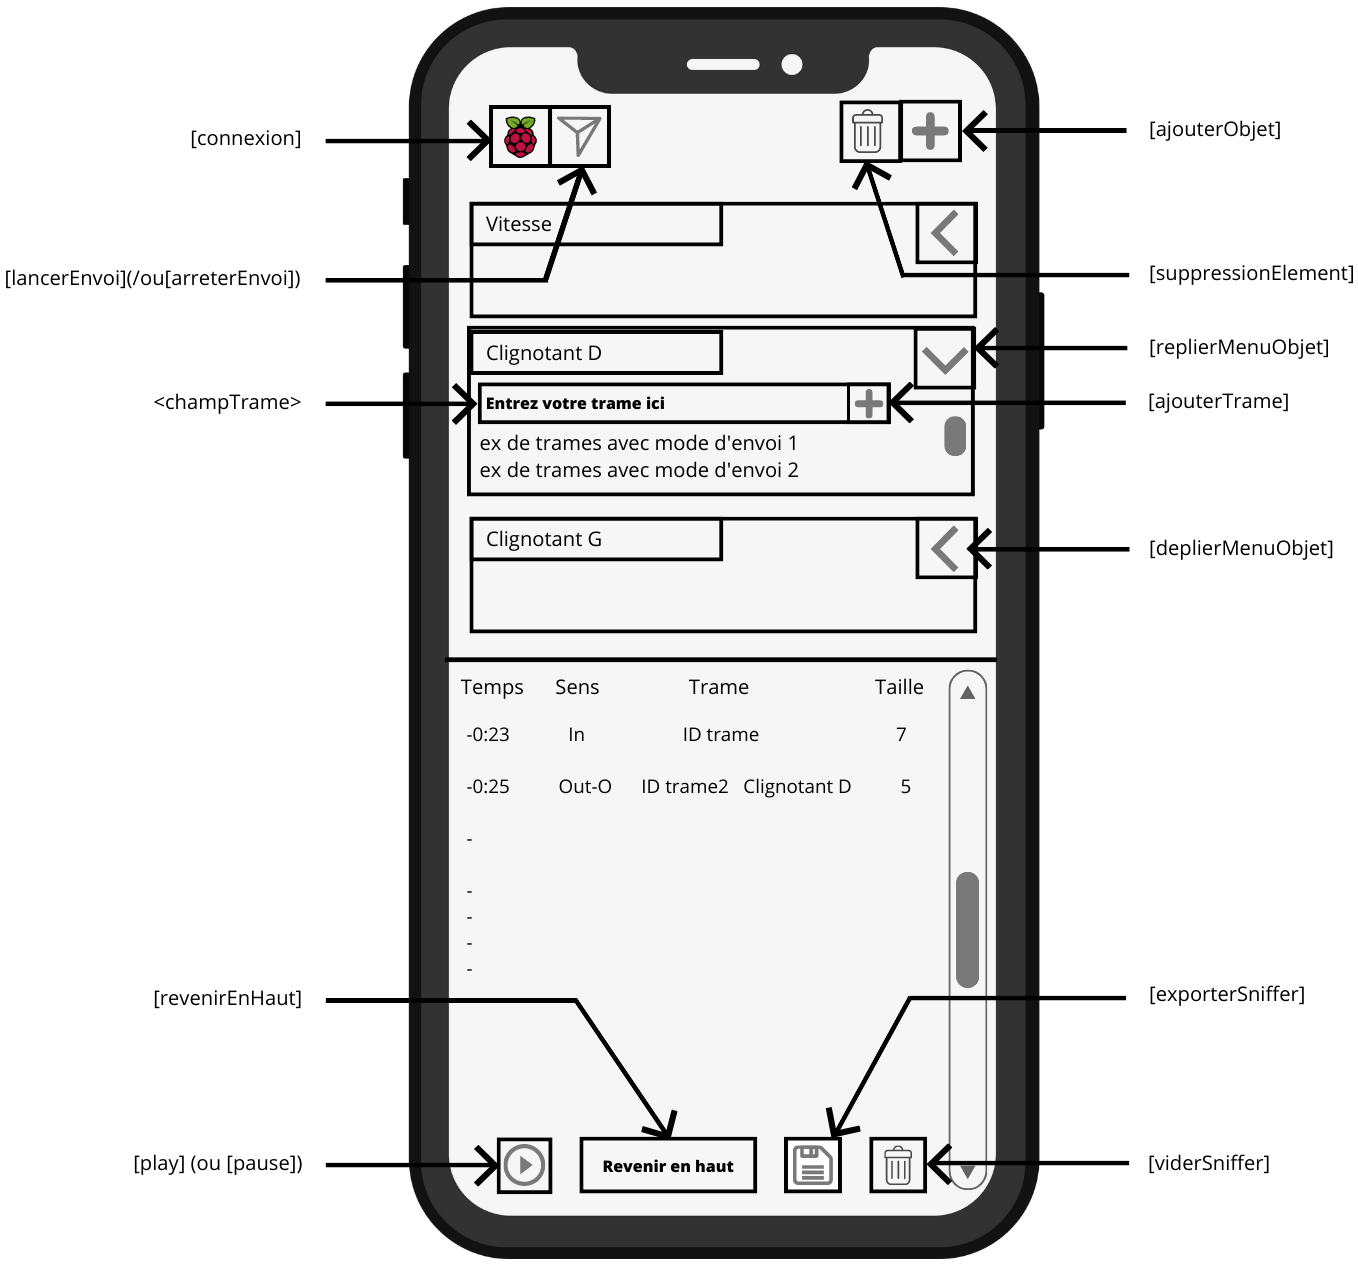
\includegraphics[width=0.85\textwidth]{sections/3_Exigences_specifiques/1_IHM/ihm/ecranPrincipalDescription.png}
    \captionof{figure}{EcranPrincipal avec légende des boutons et des champs}
    \label{ecran_boutons}
\end{minipage} \newline \medskip \medskip

L'ensemble des figures suivantes représente les noms des boutons et des champs de texte de tous les différents pop-up utilisés dans l'application {\nomApplication}. \\
\medskip

\begin{minipage}{1\linewidth}
    \centering
    
\includegraphics[width=0.91\textwidth]{sections/3_Exigences_specifiques/1_IHM/ihm/popUpObjet.png}
    \vspace{-0.3cm}
    \newline
    \captionof{figure}{PopupAjoutObjet avec nom des boutons et du champ de saisie}
    \label{ecran_ajout_objet}
\end{minipage} \newline
\vspace{1cm}

\begin{minipage}{1\linewidth}
    \centering
    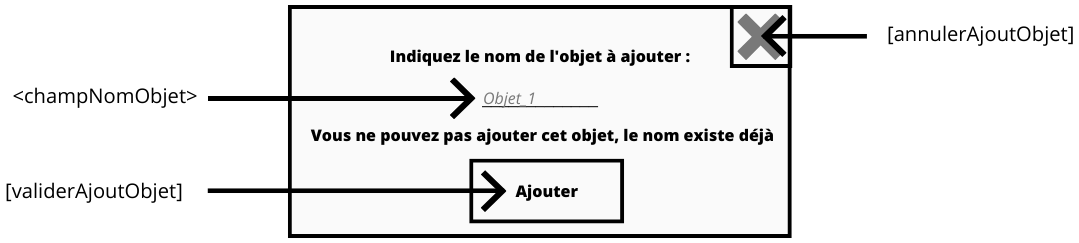
\includegraphics[width=0.91\textwidth]{sections/3_Exigences_specifiques/1_IHM/ihm/popupErreurSaisieObjet.png}
    \vspace{-0.3cm}
    \newline
    \captionof{figure}{PopupErreurAjoutObjet avec nom des boutons et du champ de saisie}
    \label{ecran_erreur_ajout_objet}
\end{minipage} \\ \\

\begin{minipage}{1.3\linewidth}
    \centering
    
\includegraphics[width=0.66\textwidth]{sections/3_Exigences_specifiques/1_IHM/ihm/popUpErreurAjoutObjet.png}
    \captionsetup{justification=centering, margin={-5cm,0cm}}
    \captionof{figure}{PopupErreurNombreObjet avec nom du bouton}
    \label{ecran_erreur_ajout_nombre_objet}
\end{minipage}\\ \\

\begin{minipage}{1\linewidth}
    \centering
    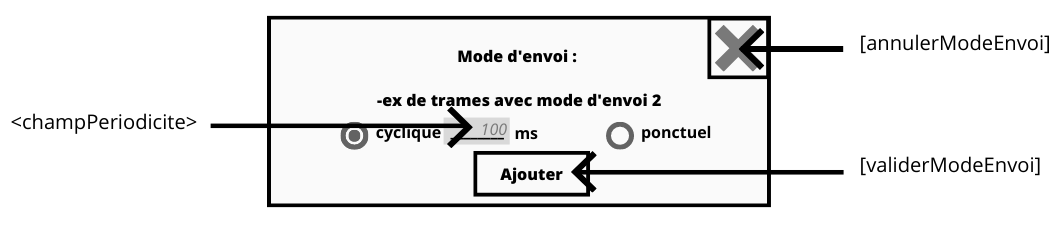
\includegraphics[width=0.93\textwidth]{sections/3_Exigences_specifiques/1_IHM/ihm/popUpTrame.png}
    \captionsetup{justification=centering, margin={1cm,0cm}}
    \captionof{figure}{PopupModeEnvoiTrame avec nom des boutons et du \newline champ de saisie de la périodicité}
    \label{ecran_mode_trame_envoi}
\end{minipage}\\ \\

\begin{minipage}{1.3\linewidth}
    \centering
    
\includegraphics[width=0.66\textwidth]{sections/3_Exigences_specifiques/1_IHM/ihm/popUpErreurTrame.png}
    \captionsetup{justification=centering, margin={-5cm,0cm}}
    \captionof{figure}{PopupErreurSaisieTrame avec nom du bouton}
    \label{ecran_erreur_saisie_trame}
\end{minipage}\\ \\

\begin{minipage}{1.3\linewidth}
    \centering
    
\includegraphics[width=0.66\textwidth]{sections/3_Exigences_specifiques/1_IHM/ihm/popUpErreurAjoutTrame.png}
    \captionsetup{justification=centering, margin={-5cm,0cm}}
    \captionof{figure}{PopupErreurNombreTrame avec nom du bouton}
    \label{ecran_erreur_ajout_nombre_trame}
\end{minipage}\\ \\

\begin{minipage}{1\linewidth}
    \centering
    
\includegraphics[width=0.91\textwidth]{sections/3_Exigences_specifiques/1_IHM/ihm/popUpArretEnvoi.png}
    \captionof{figure}{PopupArretEnvoi avec nom des boutons}
    \label{ecran_arret_envoi_trame}
\end{minipage}\\ \\

\begin{minipage}{1\linewidth}
    \centering
    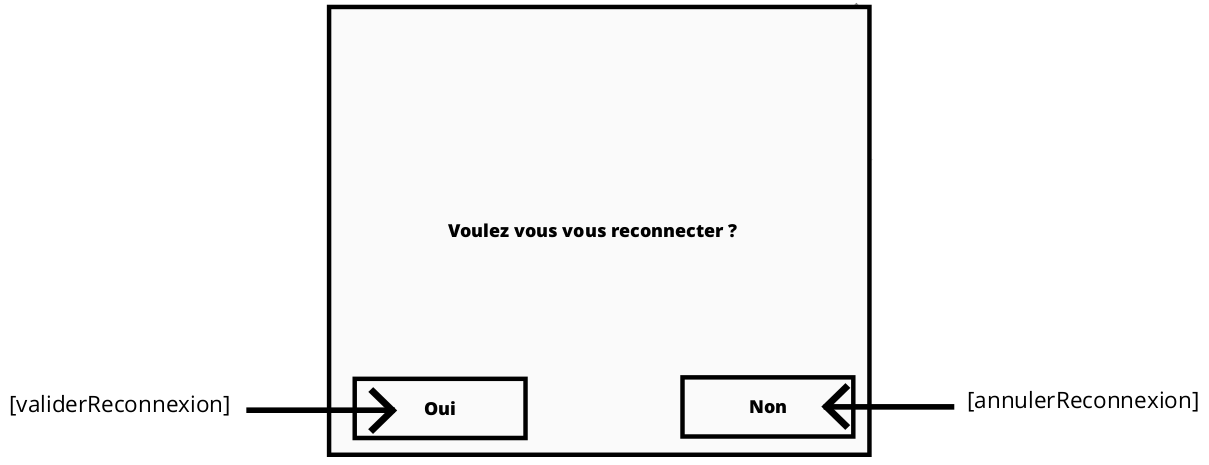
\includegraphics[width=0.9\textwidth]{sections/3_Exigences_specifiques/1_IHM/ihm/popUpReconnexion.png}
    \captionof{figure}{PopupDemandeReconnexion avec nom des boutons}
    \label{ecran_demande_reconnexion}
\end{minipage}\\ \\

\begin{minipage}{1\linewidth}
    \centering
    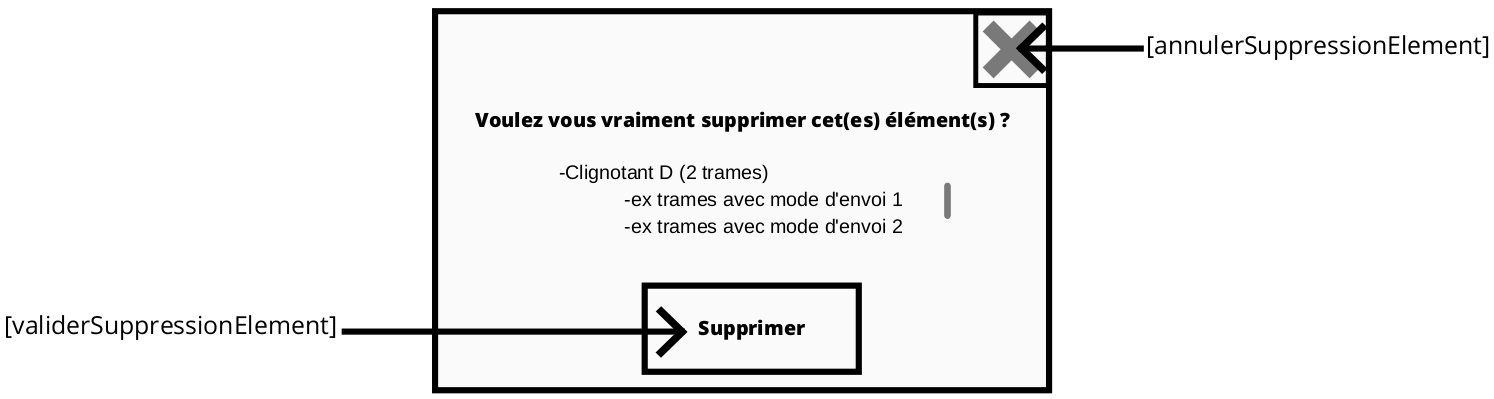
\includegraphics[width=0.9\textwidth]{sections/3_Exigences_specifiques/1_IHM/ihm/popUpSuppressionElementObjet.png}
    \captionof{figure}{PopupSuppressionElement avec nom des boutons}
    \label{ecran_suppression_element}
\end{minipage}\\

\newpage
\subsubsection{Les écrans}
\paragraph{Vue générale}

Utilisateur peut interagir avec Tableau de Bord via l'application {\nomApplication}. L'application {\nomApplication} peut transmettre des informations à Utilisateur par l'intermédiaire de l'écran du Smartphone. \newline

La figure \ref{schemaMAE} représente les navigations possibles entre les différents écrans proposés par l'IHM. Ces enchaînements sont représentés par un diagramme d'états-transitions UML. \\
Chaque écran est représenté par un état (rectangle arrondi sur la figure). Les transitions indiquées par les flèches représentent une navigation d'un écran à l'autre en précisant l'événement logique du contexte (cf. chapitre \ref{interfaces_logiques}) qui active la transition. Cela correspond généralement à des interactions de Utilisateur sur l'IHM qui génère l'événement correspondant.
\newline

Certaines transitions ne sont pas franchies sur des événements logiques, ce sont :
\begin{itemize}
    \item Les événements de temporisation (le mot-clef « after » est alors noté sur la transition) : la transition doit être sensibilisée pendant une certaine durée pour être franchie.
    \item Des conditions qui deviennent vraies (la condition est alors exprimée entre crochets).
\end{itemize}

\begin{figure}[ht] 
    \centering
    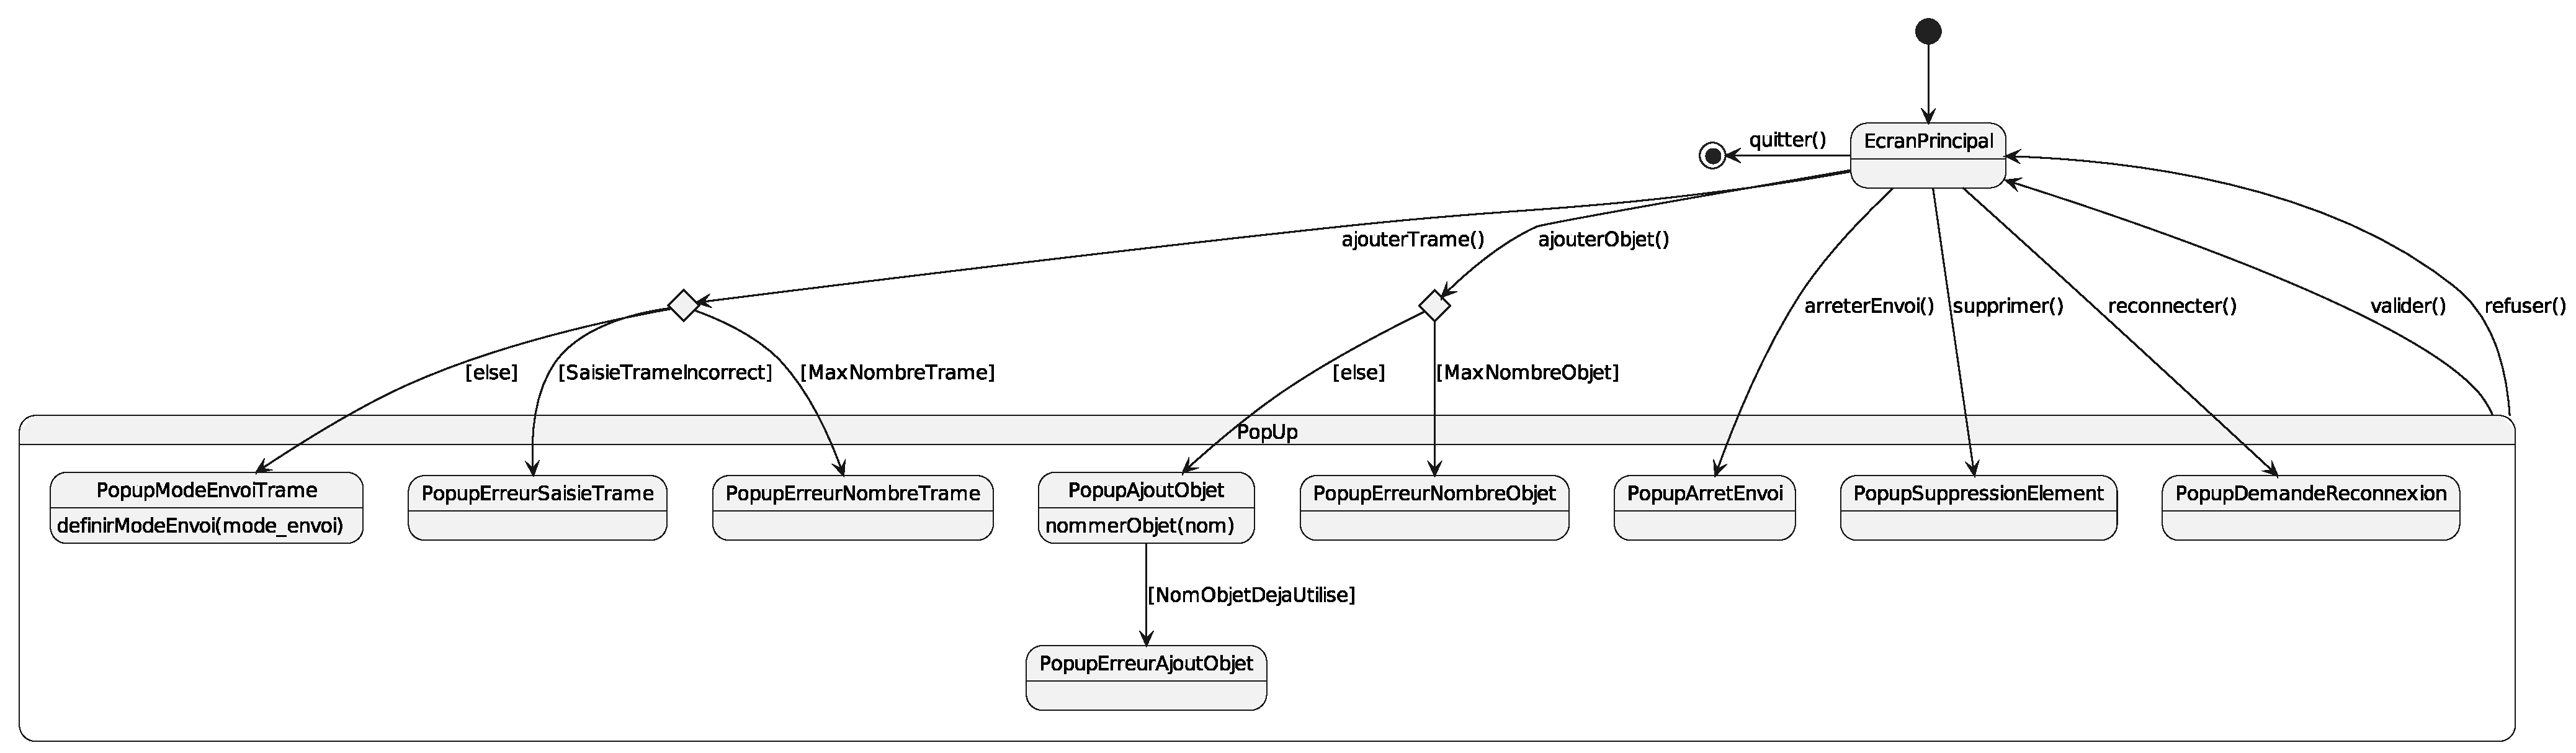
\includegraphics[width=16cm]{../schemas/MAE}
    \captionsetup{justification=centering}
    \caption{Enchaînement entre les écrans de l'IHM représenté par un diagramme états-transitions UML}
    \label{schemaMAE}
\end{figure}

\newpage

L'état initial de création de l'IHM est représenté par le disque de couleur noire. 
Après le lancement du système, l'IHM démarre avec l'écran {\guillemetleft} EcranPrincipal {\guillemetright}. 
Le disque de couleur noire entouré par un cercle correspond à la fin d'un enchaînement. 
Lorsqu'un enchaînement est fini, l'IHM s'éteint.
\newline
\newline
\`A partir de EcranPrincipal, Utilisateur peut réaliser différentes actions, qui déclencheront l'apparition de pop-up (afficherPopUp(id\_popup)). Utilisateur peut à tout moment revenir à EcranPrincipal (refuser()).
\newline
\newline
Dans le cas d'un ajout d'objet (ajouterObjet()), l'IHM affiche PopupAjoutObjet (afficherPopUp(id\_popup)). Utilisateur nomme l'objet (nommerObjet(nom)), il doit appuyer sur le bouton {\guillemetleft} Ajouter {\guillemetright} nommé [validerAjoutObjet] dans la figure \ref{ecran_ajout_objet}. Cela correspond à la fonction {\guillemetleft} valider() {\guillemetright} de la figure \ref{schemaMAE}. Si Utilisateur ne souhaite pas choisir de nom, l'application {\nomApplication} en fournit un par défaut (voir section \ref{dictionnaire}).
\newline
\newline
Dans le cas où Utilisateur saisit un nom d'objet qui est déjà utilisé par un autre objet, l'IHM affiche le pop-up d'erreur PopUpErreurAjoutObjet (afficherPopUp(id\_popup)). Ce pop-up contient une phrase qui informe Utilisateur de la source de l'erreur. Tant que Utilisateur n'aura pas modifié le nom de l'objet, il ne pourra pas l'ajouter à la liste de l'application CANdroid.
\newline
\newline
Dans le cas d'un ajout de trame (ajouterTrame()), l'IHM affiche PopupModeEnvoiTrame (afficherPopUp(id\_popup)) pour définir le mode d'envoi (definirModeEnvoi(mode\_envoi)) de la trame à ajouter. Utilisateur doit appuyer sur le bouton {\guillemetleft} Ajouter {\guillemetright} nommé [validerModeEnvoi] dans la figure \ref{ecran_mode_trame_envoi}. Cela correspond à la fonction {\guillemetleft} valider() {\guillemetright} de la figure \ref{schemaMAE} qui permet à Utilisateur de confirmer son choix.
\newline
\newline
Dans le cas où Utilisateur saisit une trame qui ne correspond pas au format utilisé par l'application CANdroid, l'IHM affiche le pop-up d'erreur PopupErreurSaisieTrame (afficherPopUp(id\_popup)). Pour fermer ce pop-up, Utilisateur doit appuyer sur le bouton [fermerErreurTrame]. Il pourra par la suite modifier le format de la trame saisie afin de pouvoir l'ajouter correctement.
\newline
\newline
Dans le cas où le nombre maximum de trames ou d'objets est atteint, l'IHM affiche respectivement les pop-ups d'erreur PopupErreurNombreTrame (afficherPopUp(id\_popup)) et PopupErreurNombreObjet (afficherPopUp(id\_popup)). Ces pop-ups contiennent un message d'erreur qui informe Utilisateur de la nature de l'erreur. Utilisateur peut simplement fermer le pop-up en cliquant sur la croix située en haut à droite. Cette action le ramènera sur EcranPrincipal. Dans la figure \ref{ecran_erreur_ajout_nombre_trame}, la croix est identifiée par [fermerErreurNombreTrame], tandis que dans la figure \ref{ecran_erreur_ajout_nombre_objet} elle est identifiée par [fermerErreurNombreObjet].
\newpage
Dans le cas d'une suppression d'élément (supprimer()), l'IHM affiche PopupSuppressionElement (afficherPopUp(id\_popup)). Le pop-up affiche la liste des éléments sélectionnés, Utilisateur doit appuyer sur le bouton {\guillemetleft} Supprimer {\guillemetright} nommé [validerSuppressionElement] dans la figure \ref{ecran_suppression_element}. Cela correspond à la fonction {\guillemetleft} valider() {\guillemetright} de la figure \ref{schemaMAE} qui permet à Utilisateur de confirmer son choix.
\newline
\newline
Dans le cas d'un arrêt de l'envoi de trames (arreterEnvoiTrames()), l'IHM affiche PopupArretEnvoi (afficherPopUp(id\_popup)). Utilisateur doit appuyer sur le bouton {\guillemetleft} Oui {\guillemetright} nommé [validerArretEnvoi] dans la figure \ref{ecran_arret_envoi_trame}, ou sur le bouton {\guillemetleft} Non {\guillemetright} nommé [annulerArretEnvoi] dans la même figure. Cela correspond respectivement aux fonctions {\guillemetleft} valider() {\guillemetright} et {\guillemetleft} refuser() {\guillemetright} de la figure \ref{schemaMAE} qui permet à Utilisateur de confirmer ou annuler son choix.
\newline
\newline
Dans le cas d'une perte de connexion, si Utilisateur souhaite se reconnecter (reconnecter()), l'IHM affiche PopupDemandeReconnexion(afficherPopUp(id\_popup)). Utilisateur choisit de se reconnecter en appuyant sur le bouton {\guillemetleft} Oui {\guillemetright} nommé [validerReconnexion] dans la figure \ref{ecran_demande_reconnexion}, ou sur le bouton {\guillemetleft} Non {\guillemetright} nommé [annulerReconnexion] dans la même figure. Cela correspond respectivement aux fonctions {\guillemetleft} valider() {\guillemetright} et {\guillemetleft} refuser() {\guillemetright} de la figure \ref{schemaMAE} qui permet à Utilisateur de confirmer ou annuler son choix.

\newpage
\paragraph{EcranPrincipal}

\vspace{1cm}
\begin{minipage}{1\linewidth}
    \centering
    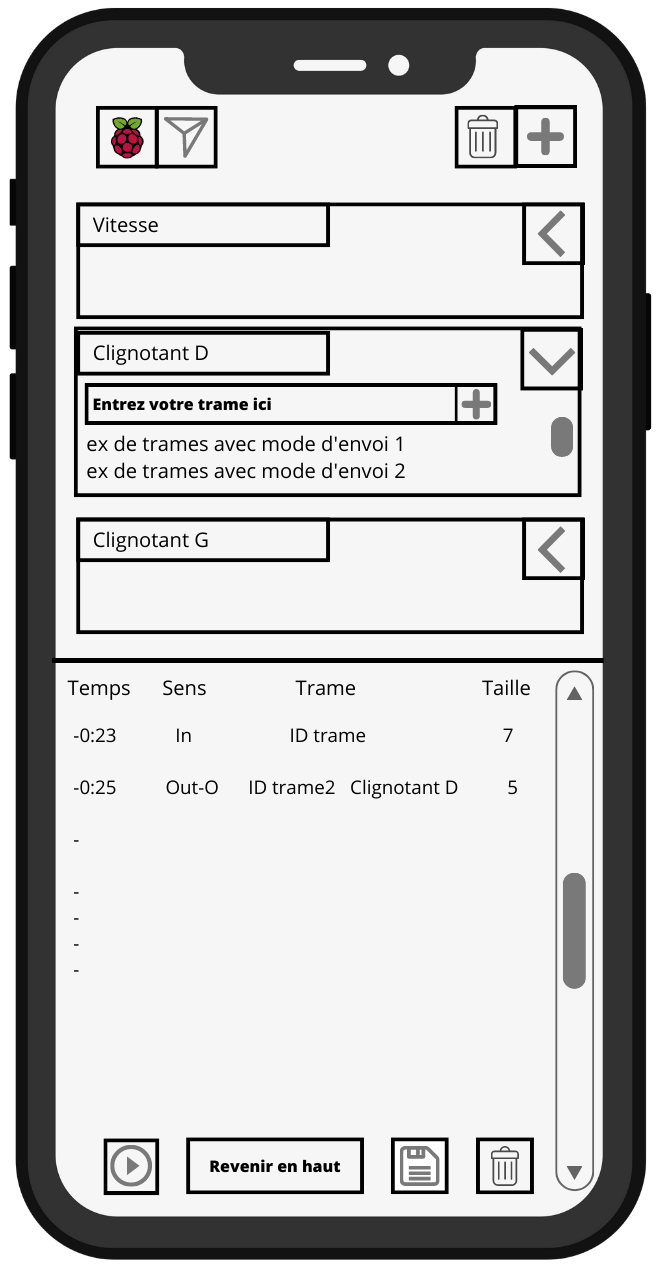
\includegraphics[width=0.45\textwidth]{sections/3_Exigences_specifiques/1_IHM/ihm/ecranPrincipal.png}
    \captionsetup{justification=centering}
    \captionof{figure}{Affichage général de EcranPrincipal}
    \label{ecran_principal}
\end{minipage}\hfill
\newline
\newline
EcranPrincipal se décompose en deux parties. La partie haute permet de déclencher des interactions avec Tableau de Bord tandis que la partie basse correspond au sniffer CAN.
\medskip

\newpage
\paragraph{Partie haute de l'écran}
\medskip
La partie {\guillemetleft} envoi {\guillemetright} (partie haute de l'écran) permet d'intéragir avec Tableau de Bord. On y observe l'état de la connexion au programme {\nomLogiciel}. On peut ajouter ou supprimer des objets, et dans ces mêmes objets, ajouter ou supprimer des trames. Enfin, on peut y ordonner l'envoi de trames. 
\newline
\newline
\textbf{Connexion : } \\

Lors du démarrage de l'application {\nomApplication}, la connexion avec le programme {\nomLogiciel} s'initialise automatiquement et continue en tâche de fond de l'application. Une connexion valide est représentée par l'icône de framboise (bouton [connexion]) en haut à gauche. Si la connexion ne s'est pas correctement déroulée, l'icône est grisée et barrée. Ainsi, au lancement de l'application {\nomApplication}, l'icône est d'abord grisée et barrée (voir figure \ref{ecran_principal_non_connecte}), puis, elle se colore si la connexion aboutit en moins de 3 secondes (voir figure \ref{ecran_sans_objet}). Si la connexion n'aboutit pas, Utilisateur peut demander à recommencer en cliquant sur le bouton [connexion] (dont l'icône est grisée et barrée). Un pop-up s'affiche et demande si l'on souhaite une reconnexion ou non au programme {\nomLogiciel} (voir figure \ref{ecran_principal_demande_reconnexion}). L'application {\nomApplication} peut être utilisée sans connexion. Dans ce cas, l'icône de framboise reste grisée et barrée. Le bouton [lancerEnvoi] est de couleur noire sur fond gris foncé pour indiquer qu'il est impossible d'envoyer des trames sur le bus CAN. De même pour le sniffer où le bouton [play] n'est pas cliquable. S'il est vide alors un message nous informe qu'il n'y a pas de trames sur le bus (voir figure \ref{ecran_principal_non_connecte}). 

\begin{minipage}{0.5\linewidth}
    \centering
    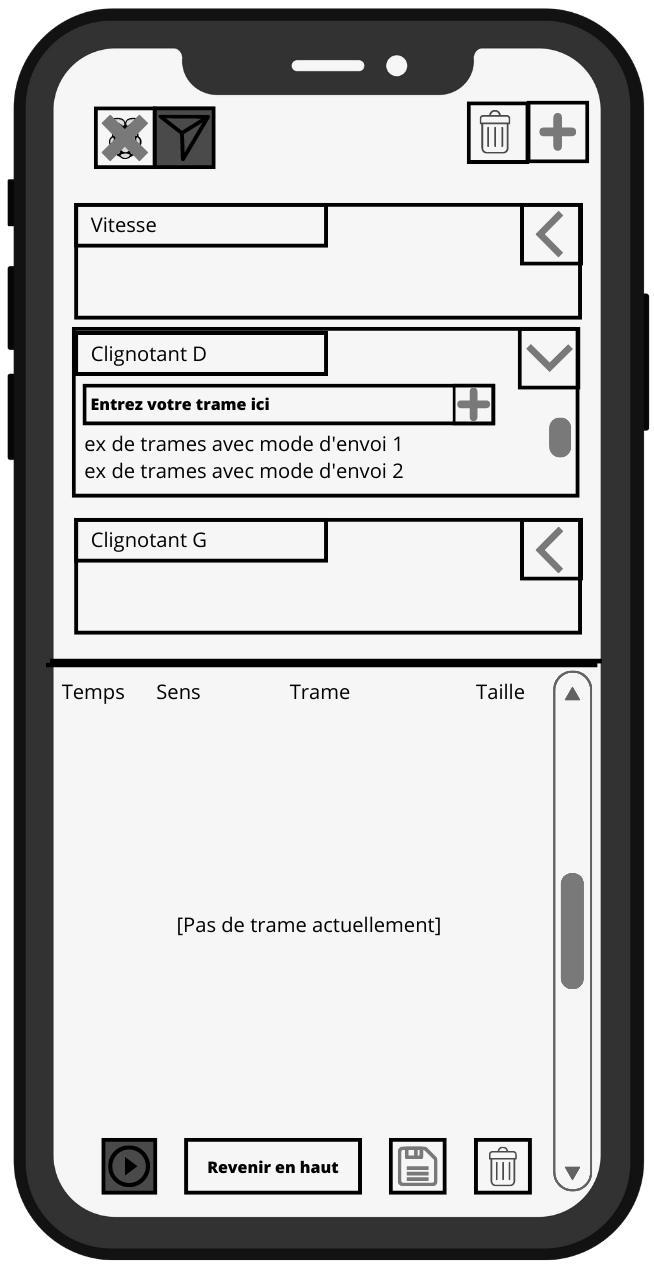
\includegraphics[width=0.7\textwidth]{sections/3_Exigences_specifiques/1_IHM/ihm/ecranPrincipalNonCo.png}
    \captionsetup{justification=centering}
    \captionof{figure}{Affichage de EcranPrincipal \newline non connecté}
    \label{ecran_principal_non_connecte}
\end{minipage}\hfill
\begin{minipage}{0.5\linewidth}
    \centering
    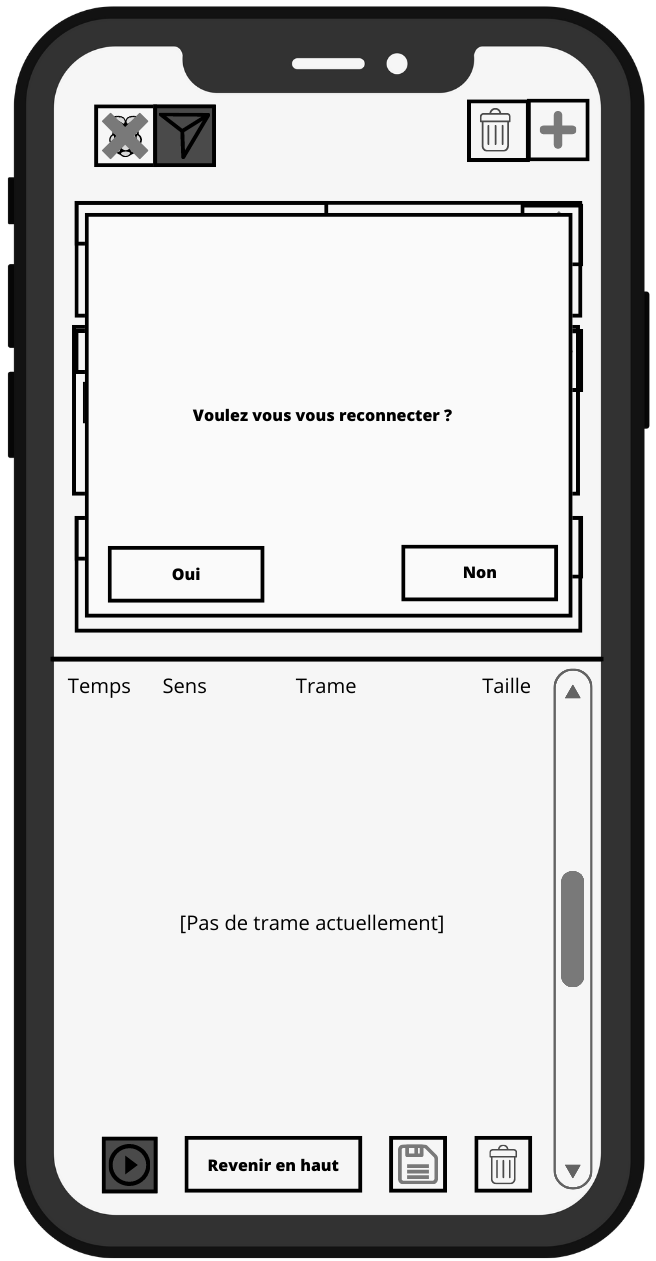
\includegraphics[width=0.7\textwidth]{sections/3_Exigences_specifiques/1_IHM/ihm/ecranReconnexion.png}
    \captionsetup{justification=centering}
    \captionof{figure}{Affichage de PopupDemandeReconnexion}\label{ecran_principal_demande_reconnexion}
\end{minipage}

\newpage
\textbf{Objet : } \\
\newline
Les objets sont matérialisés sur l'application {\nomApplication} par un rectangle (voir figure \ref{ecran_principal}). Ce rectangle comprend un sous-rectangle avec le nom de l'objet en haut à gauche et, à droite, une flèche déroule le menu de l'objet (bouton [deplierMenuObjet] ou [replierMenuObjet] pour l'effet inverse) pour afficher les trames déjà ajoutées dans cet objet. \newline \\
Les objets sont conservés d'une utilisation à l'autre sur l'application {\nomApplication}. Ils sont triés du plus récent en haut au plus ancien.
Lorsqu'il n'y a pas d'objet, un texte l'indique par un message d'information (voir figure \ref{ecran_sans_objet}). 
\vspace{0.5cm}

\begin{minipage}{0.9\linewidth}
    \centering
    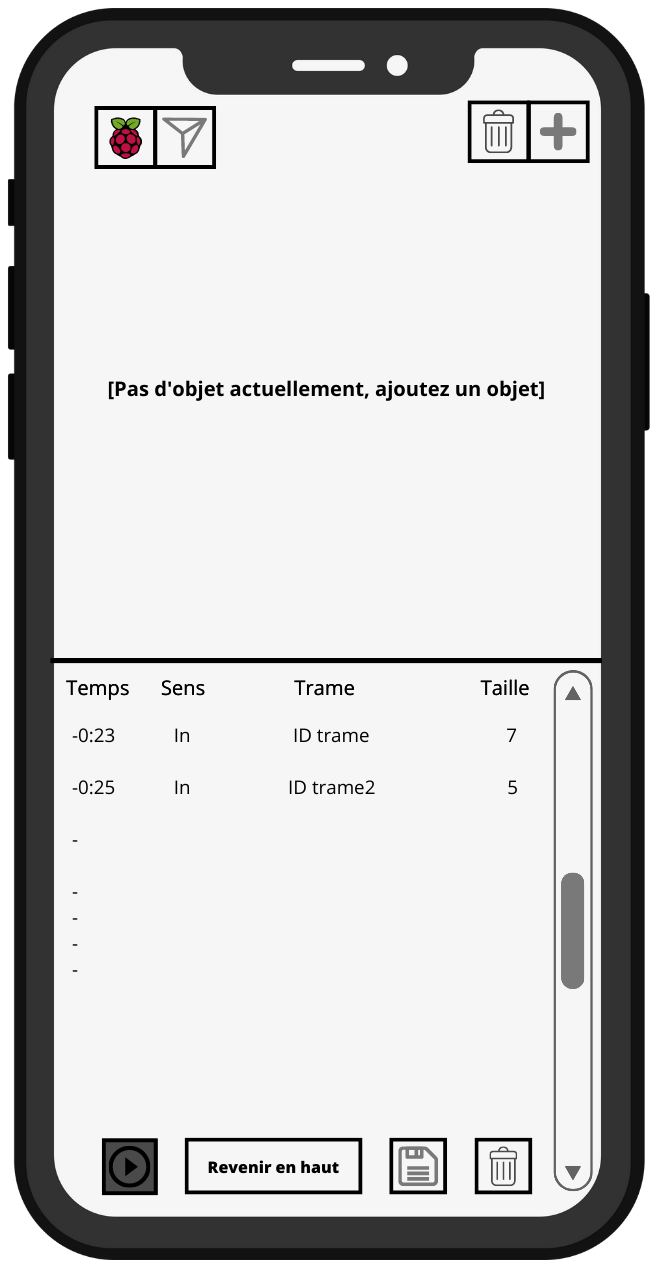
\includegraphics[width=0.5\textwidth]{sections/3_Exigences_specifiques/1_IHM/ihm/ecranPrincipalSansObjet.png}
    \captionof{figure}{Affichage de EcranPrincipal sans objet}
    \label{ecran_sans_objet}
\end{minipage}\hfill 

\newpage

L'ajout d'objet se concrétise en cliquant sur l'icône {\guillemetleft} + {\guillemetright} (bouton [ajouterObjet]) en haut à droite de l'écran. PopupAjoutObjet s'affiche alors pour que Utilisateur insère un nouveau nom d'objet (voir figure \ref{ecran_creation_objet}). Lorsque le nom est entré, Utilisateur clique sur {\guillemetleft} Ajouter {\guillemetright} (bouton [validerAjoutObjet]) pour valider l'ajout de l'objet et l'afficher automatiquement dans la liste des objets présents sur l'application {\nomApplication}. \newline \\ 
Si Utilisateur ne remplit pas le champ du nom d'objet lors de la création d'un nouvel objet dans l'application {\nomApplication}, celle-ci va automatiquement créer un objet avec un nom d'objet par défaut prérempli. Ce nom d'objet par défaut est visible en italique et en gris dans le champ nommé <champNomObjet> (voir section \ref{dictionnaire}). \\

\begin{minipage}{1\linewidth}
    \centering
    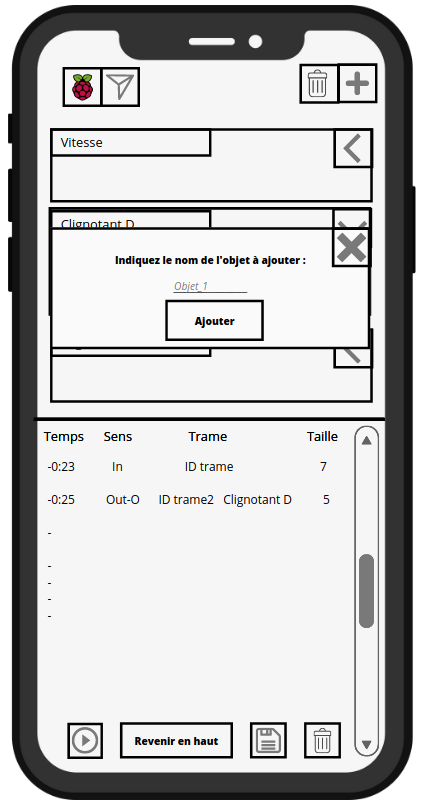
\includegraphics[width=0.5\textwidth]{sections/3_Exigences_specifiques/1_IHM/ihm/ecranCreationObjet.png}
    \captionof{figure}{Affichage de PopupAjoutObjet}
    \label{ecran_creation_objet}
\end{minipage}\hfill 

\newpage

Cependant, Utilisateur ne peut pas utiliser un nom déjà existant lorsqu'il ajoute un objet. Si le nom est déjà pris, un message d'erreur {\guillemetleft} Vous ne pouvez pas ajouter cet objet, le nom existe déjà {\guillemetright} s'affiche (voir figure \ref{ecran_creation_erreur_objet}). \newline \\ De plus, Utilisateur est limité dans le nombre d'objets qu'il peut créer sur l'application CANdroid. Si cette limite est atteinte et que Utilisateur souhaite ajouter un nouvel objet, une fenêtre d'erreur appelée PopupErreurNombreObjet s'affichera (voir figure \ref{ecran_principal_popup_erreur_nombre_objet}). \\\\

\begin{minipage}{0.5\linewidth}
    \centering
    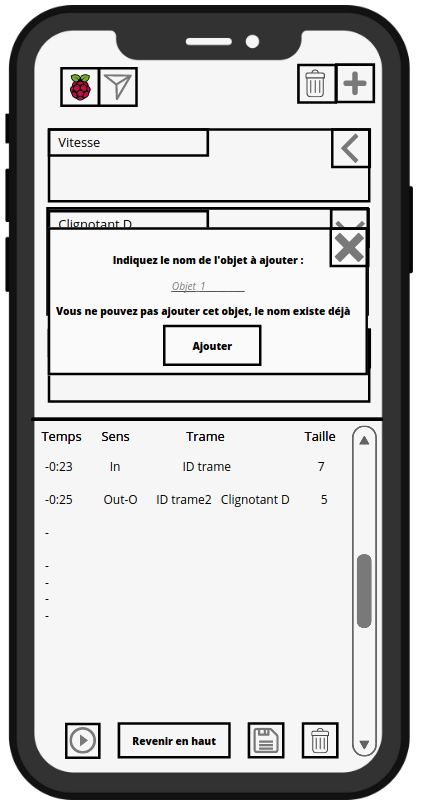
\includegraphics[width=0.7\textwidth]{sections/3_Exigences_specifiques/1_IHM/ihm/ecranCreationObjetErreur.png}
    \captionsetup{justification=centering}
    \captionof{figure}{Affichage de PopupErreurAjoutObjet}
    \label{ecran_creation_erreur_objet}
\end{minipage} \hfill
\begin{minipage}{0.5\linewidth}
    \centering
    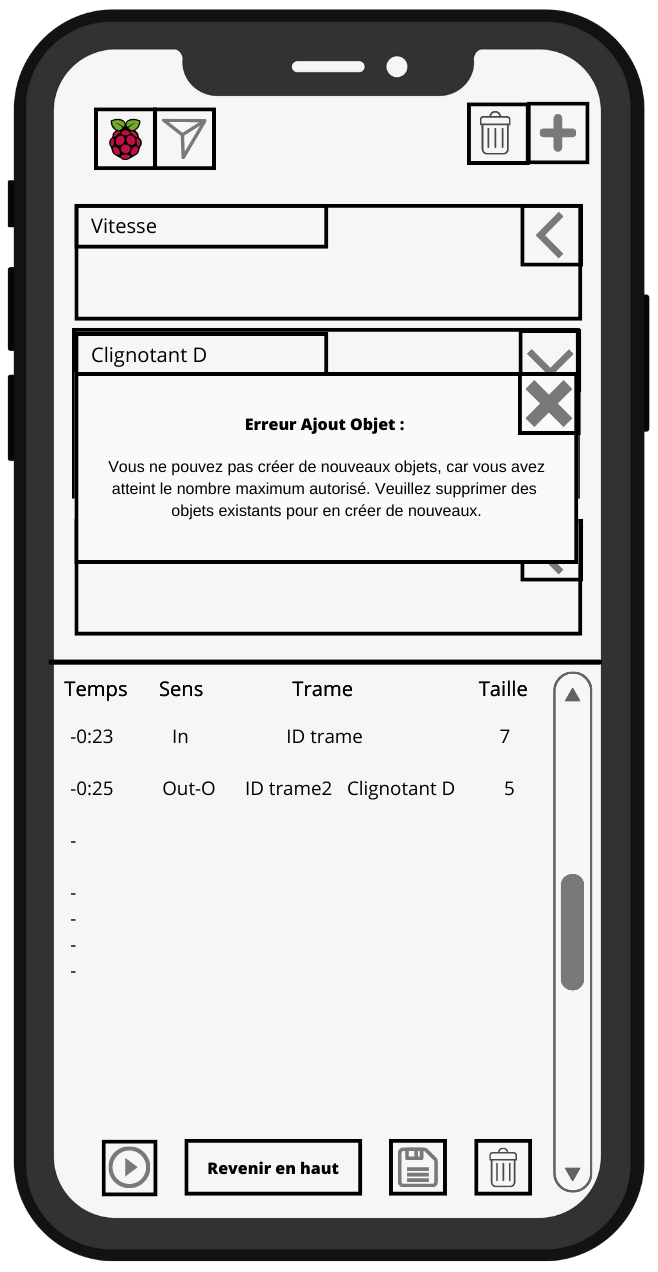
\includegraphics[width=0.7\textwidth]{sections/3_Exigences_specifiques/1_IHM/ihm/ecranErreurNombreObjet.png}
    \captionsetup{justification=centering}
    \captionof{figure}{Affichage de \newline PopupErreurNombreObjet}
    \label{ecran_principal_popup_erreur_nombre_objet}
\end{minipage} 

\newpage

Pour supprimer un objet, Utilisateur clique sur l'objet, la case entière se grise puis Utilisateur clique sur la poubelle en haut à droite de EcranPrincipal (bouton [suppressionElement] sur la figure \ref{ecran_objet_selectionne}). PopupSuppressionElement s'affiche pour demander confirmation à Utilisateur. La suppression d'un objet entraîne la suppression des trames associées à cet objet. La liste des éléments sélectionnés à supprimer est indiquée sur le pop-up et Utilisateur clique sur {\guillemetleft} Supprimer {\guillemetright} (bouton [validerSuppressionElement]) pour valider la suppression (voir figure \ref{ecran_suppression_element}).
 
\vspace{0.5cm}
\begin{minipage}{0.5\linewidth}
    \centering
    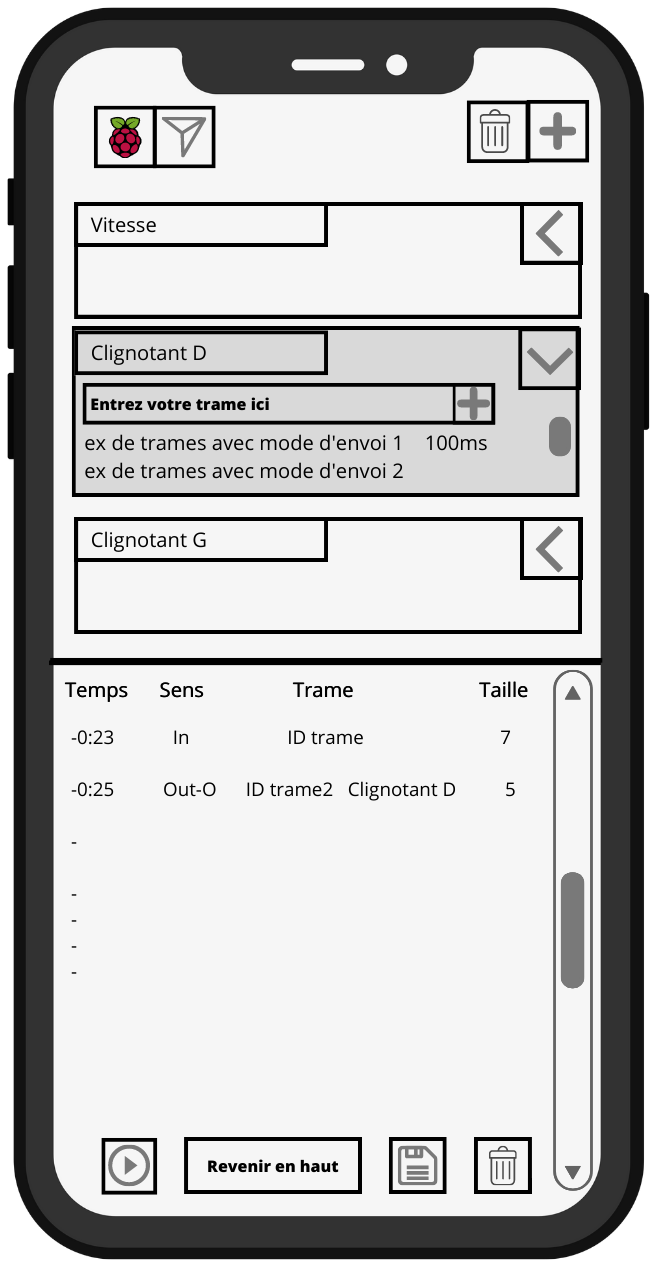
\includegraphics[width=0.7\textwidth]{sections/3_Exigences_specifiques/1_IHM/ihm/ecranPrincipalSelectionObjet.png}
    \captionsetup{justification=centering}
    \captionof{figure}{Affichage de EcranPrincipal\newline avec l'objet {\guillemetleft} Clignotant D {\guillemetright} sélectionné} \label{ecran_objet_selectionne}
\end{minipage}\hfill
\begin{minipage}{0.5\linewidth}
    \centering
    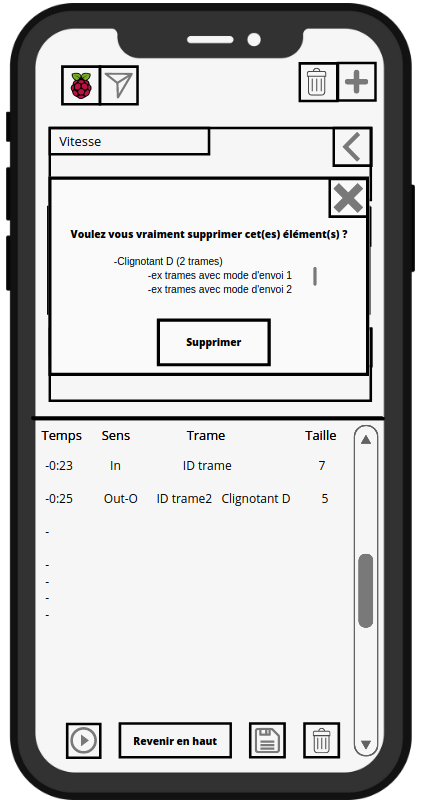
\includegraphics[width=0.7\textwidth]{sections/3_Exigences_specifiques/1_IHM/ihm/ecranSuppressionElementObjet.png}
    \captionsetup{justification=centering}
    \captionof{figure}{Affichage de PopupSuppressionElement} \label{ecran_popup_suppression_element}
\end{minipage} \newline 

\newpage
\textbf{Trames : } \\

Chaque trame est associée à un objet. Les trames sont visibles dans le rectangle de l'objet associé à la suite du nom de l'objet et dans l'ordre de leur ajout. Si possible, la trame est affichée dans sa globalité. Une trame possède un mode d'envoi : cyclique ou ponctuel. 
Pour visualiser la liste des trames, Utilisateur clique sur la flèche de l'objet (bouton [deplierMenuObjet]) pour dérouler le menu de l'objet et ainsi voir ses trames. Voir sur la figure \ref{ecran_principal} où le menu de l'objet {\guillemetleft} Clignotant D {\guillemetright} est déroulé et on peut y voir ses trames, contrairement à l'objet {\guillemetleft} Vitesse {\guillemetright}. \newline

\begin{minipage}{0.5\linewidth}
    \centering
    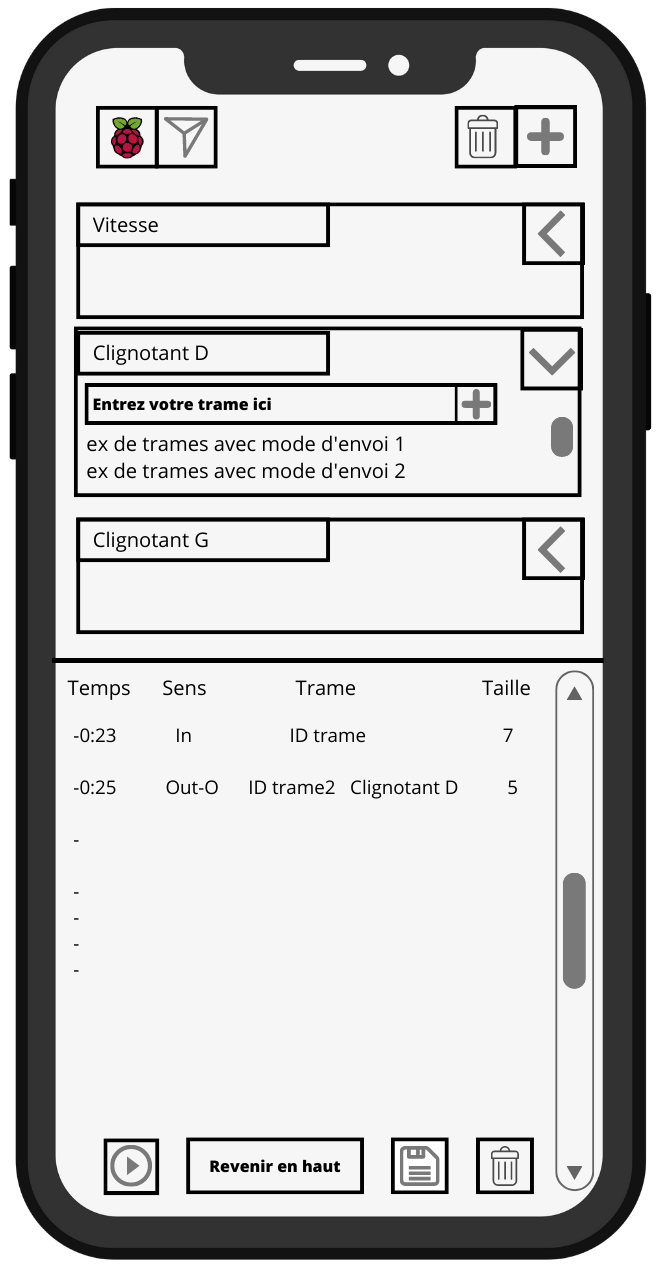
\includegraphics[width=0.7\textwidth]{sections/3_Exigences_specifiques/1_IHM/ihm/ecranPrincipal.png}
    \captionsetup{justification=centering}
    \captionof{figure}{Affichage de EcranPrincipal\newline pour la saisie de trames} 
    \label{ecran_principal_ajout_trame}
\end{minipage}\hfill
\begin{minipage}{0.5\linewidth}
    \centering
    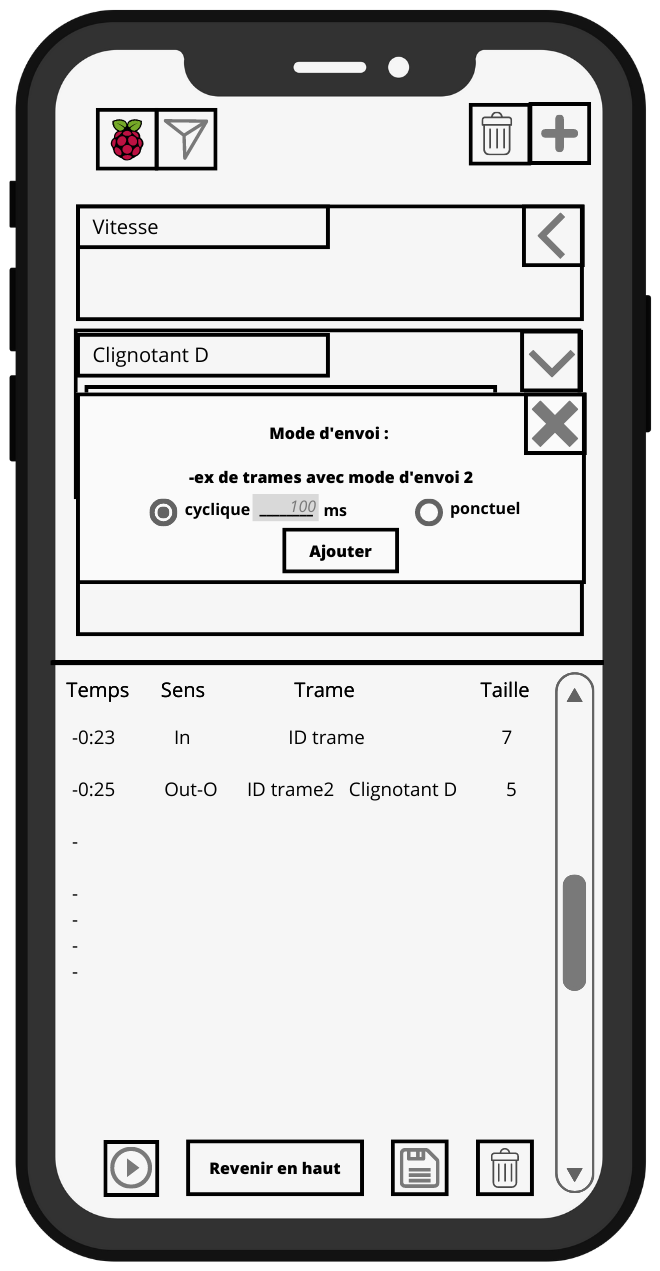
\includegraphics[width=0.7\textwidth]{sections/3_Exigences_specifiques/1_IHM/ihm/ecranModeEnvoiTrame.png}
    \captionsetup{justification=centering}
    \captionof{figure}{Affichage de PopupModeEnvoiTram} 
    \label{ecran_mode_envoi_trames}
\end{minipage} \newline 

\vspace{0.5cm}

Pour ajouter une nouvelle trame, Utilisateur se place dans l'objet auquel il veut l'associer. Il saisit la trame sous le format {\guillemetleft} \#id\$size\@@message {\guillemetright} dans champ <champTrame>. C'est à Utilisateur d'écrire à la main les séparateurs. Cette syntaxe permet d'éviter à Utilisateur d'écrire les zéros non-significatifs. Utilisateur clique ensuite sur le bouton [ajouterTrame]. Si Utilisateur ne saisit pas la trame sous le bon format, PopupErreurSaisieTrame s'affiche (voir figure \ref{ecran_principal_popup_erreur_saisie_trame}). Tant que Utilisateur ne saisit pas une trame sous le bon format, l'ajout ne pourra pas se faire.
\newline \\
Lorsque Utilisateur entre le bon format défini précédemment pour les trames, PopupModeEnvoiTrame s'ouvre (voir figure \ref{ecran_mode_envoi_trames}) et demande à Utilisateur de choisir le mode d'envoi de la trame, pour cela, il doit cliquer sur le bouton radio correspondant au mode d'envoi souhaité. Un radio bouton est un élément qui permet à Utilisateur de sélectionner le mode d'envoi ponctuel (bouton [radioBoutonPonctuel]) ou le mode d'envoi cyclique (bouton [radioBoutonCyclique]). Lorsqu'un bouton radio est sélectionné, le cercle le définissant se remplit, et l'autre bouton radio est automatiquement désélectionné, le cercle le définissant se vide. Par défaut, une trame est périodique de périodicité 100ms mais Utilisateur peut la modifier grâce au champ <champPeriodicite>. Utilisateur clique sur {\guillemetleft} Ajouter {\guillemetright} (bouton [validerModeEnvoi]) pour valider l'ajout de la trame (voir figure \ref{ecran_mode_envoi_trames}). \newline

De la même manière que pour l'ajout d'objets, il existe également une limite pour le nombre de trames que Utilisateur peut ajouter. Si cette limite est atteinte et que Utilisateur tente d'ajouter une nouvelle trame, PopupErreurNombreTrame s'affiche (voir figure \ref{ecran_principal_popup_erreur_nombre_trame}).
\newline \\

\begin{minipage}{0.5\linewidth}
    \centering
    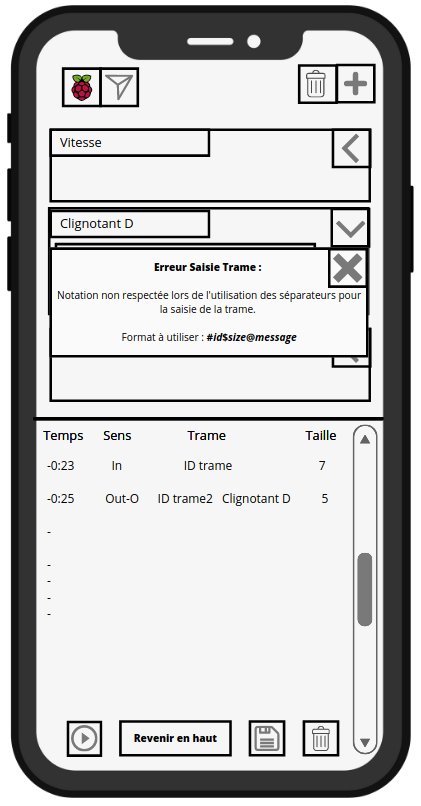
\includegraphics[width=0.7\textwidth]{sections/3_Exigences_specifiques/1_IHM/ihm/ecranErreurTrame.png}
    \captionsetup{justification=centering}
    \captionof{figure}{Affichage de\newline PopupErreurSaisieTrame} 
    \label{ecran_principal_popup_erreur_saisie_trame}
\end{minipage}\hfill
\begin{minipage}{0.5\linewidth}
    \centering
    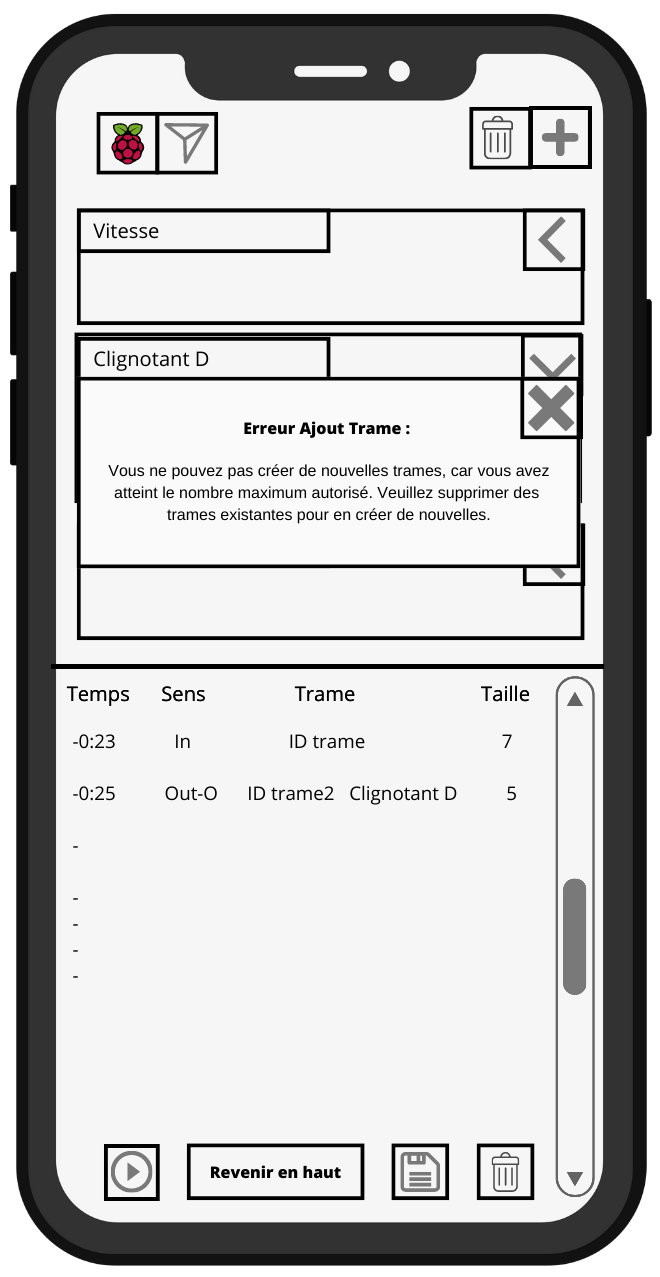
\includegraphics[width=0.7\textwidth]{sections/3_Exigences_specifiques/1_IHM/ihm/ecranErreurNombreTrame.png}
    \captionsetup{justification=centering}
    \captionof{figure}{Affichage de PopupErreurNombreTrame} 
    \label{ecran_principal_popup_erreur_nombre_trame}
\end{minipage} \newline 

\newpage

Pour envoyer une trame, Utilisateur clique sur une trame à envoyer. S'il souhaite en envoyer plusieurs, la sélection est successive. Une trame est considérée comme sélectionnée si elle est grisée claire (voir figure \ref{ecran_trame_selectionne}). Si Utilisateur souhaite désélectionner une trame, il lui suffit de re-cliquer dessus. Lorsque la sélection est effectuée, Utilisateur clique sur l'icône d'envoi en haut à gauche de l'écran (bouton [lancerEnvoi]). Une trame en cours d'envoi se distingue par un surlignage gris foncé et l'écriture en blanc (voir figure \ref{ecran_trame_envoi}). Le bouton d'envoi est également blanc sur fond gris foncé pour indiquer que des trames sont en cours d'envoi. Dans cet état-là, les boutons de suppression et d'ajout (trames comme objets) sont en noir sur fond gris foncé pour montrer que les outils correspondants sont désactivés.
\\\\
\vspace{2cm}
\begin{minipage}{0.5\linewidth}
    \centering
    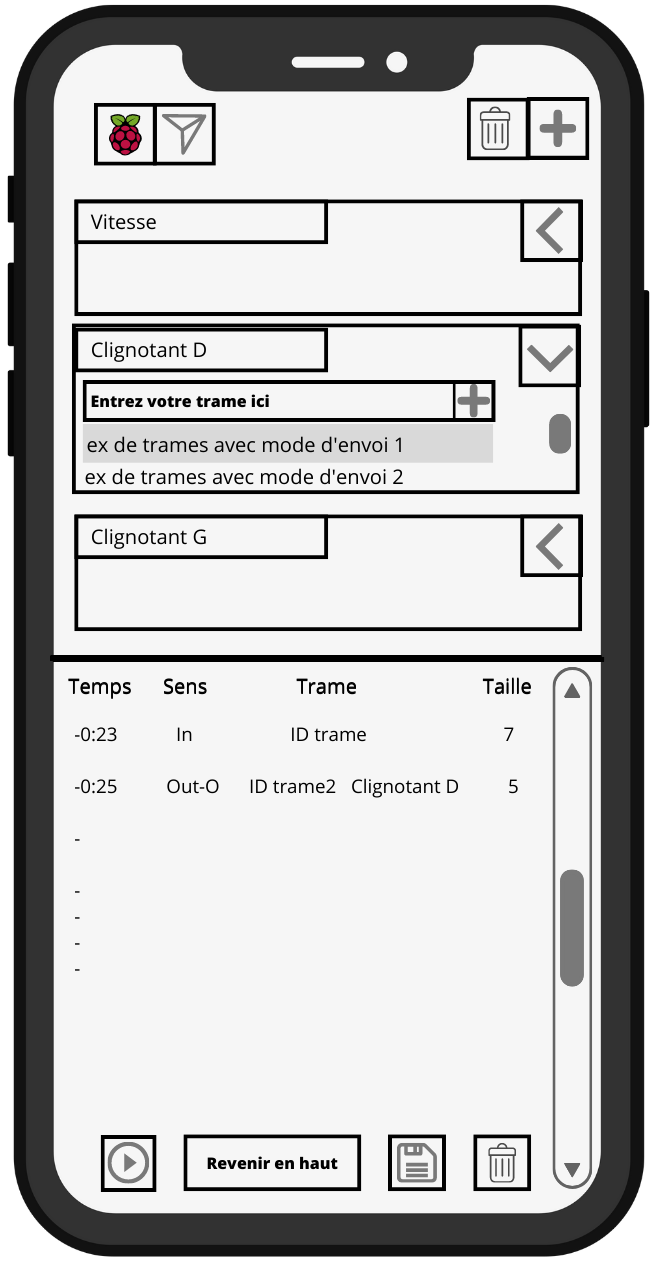
\includegraphics[width=0.7\textwidth]{sections/3_Exigences_specifiques/1_IHM/ihm/ecranPrincipalSelectionTrame.png}
    \captionsetup{justification=centering}
    \captionof{figure}{Affichage de EcranPrincipal\newline avec  une trame de l'objet {\guillemetleft} Clignotant D {\guillemetright} sélectionnée}
    \label{ecran_trame_selectionne}
\end{minipage}\hfill
\begin{minipage}{0.5\linewidth}
    \centering
    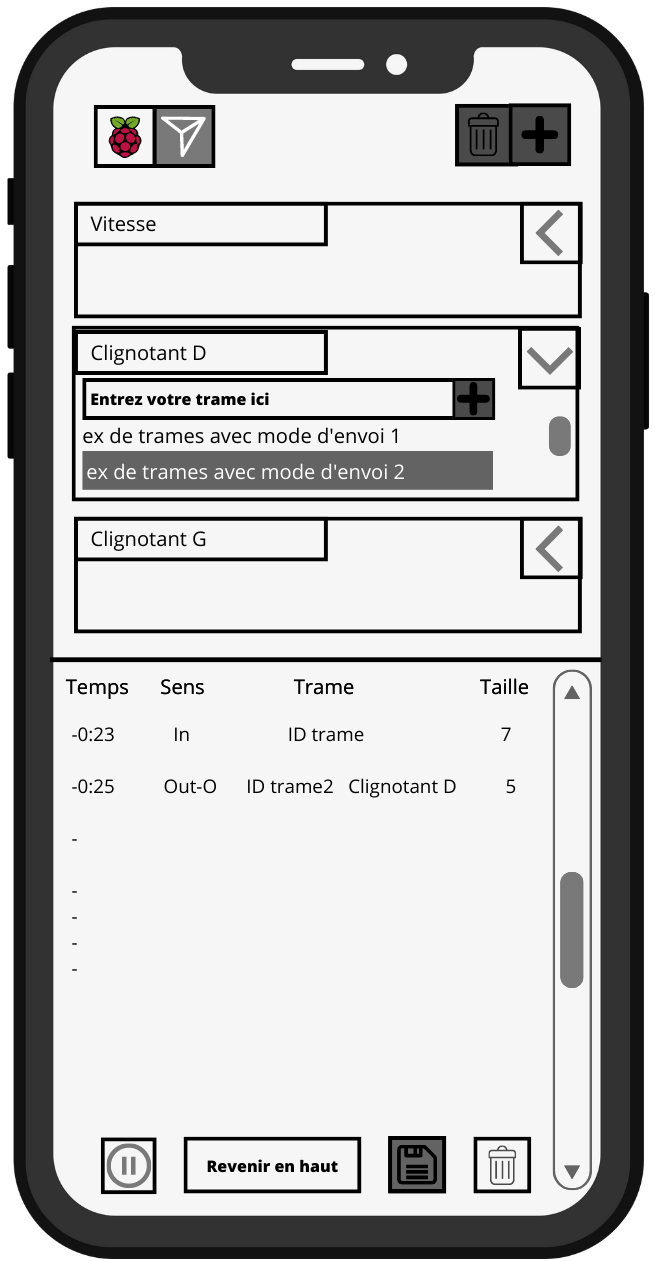
\includegraphics[width=0.7\textwidth]{sections/3_Exigences_specifiques/1_IHM/ihm/ecranPrincipalTrameEnCours.png}
    \captionsetup{justification=centering}
    \captionof{figure}{Affichage de EcranPrincipal lorsque des trames sont en cours d'envoi}
    \label{ecran_trame_envoi}
\end{minipage} \newline 
\vspace{1cm}

\newpage
Pour arrêter l'envoi des trames, Utilisateur clique à nouveau sur le bouton d'envoi (bouton [arreterEnvoi]), PopupArretEnvoi apparaît pour demander la confirmation à Utilisateur (voir figure \ref{ecran_arret_envoi}). Utilisateur valide ce changement d'état en cliquant sur {\guillemetleft} Oui {\guillemetright} (bouton [validerArretEnvoi]), dans le cas inverse Utilisateur clique sur {\guillemetleft} Non {\guillemetright} (bouton [annulerArretEnvoi]) et le mode d'envoi continue. 
\\\\
\begin{minipage}{1\linewidth}
    \centering
    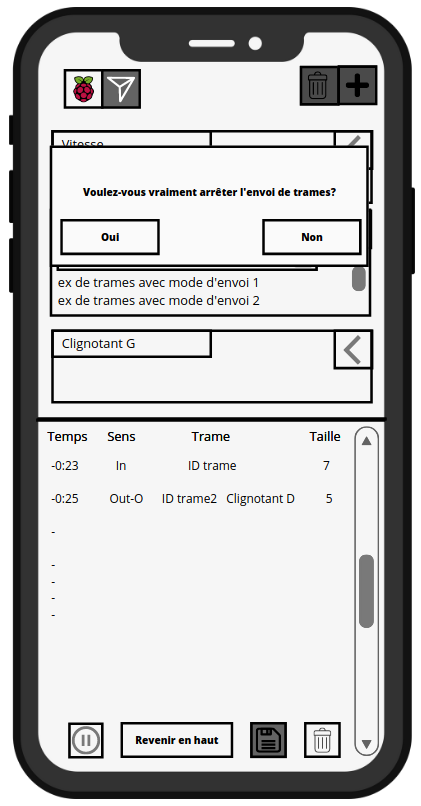
\includegraphics[width=0.48\textwidth]{sections/3_Exigences_specifiques/1_IHM/ihm/ecranArretEnvoi.png}
    \captionof{figure}{Affichage de PopupArretEnvoi}
    \label{ecran_arret_envoi}
\end{minipage}\hfill

\newpage
De même que pour supprimer un objet, pour supprimer une trame, Utilisateur clique sur la trame qu'il souhaite supprimer, la ligne se grise puis Utilisateur clique sur la poubelle (bouton [suppressionElement]) en haut à droite de EcranPrincipal (voir figure \ref{ecran_trame_selectionne}). La liste des éléments sélectionnés à supprimer est indiquée sur PopupSuppressionElement et Utilisateur clique sur {\guillemetleft} Supprimer {\guillemetright} (bouton [validerSuppressionElement]) pour valider la suppression (voir figure \ref{ecran_suppression_trames}).
\\\\
\begin{minipage}{1\linewidth}
    \centering
    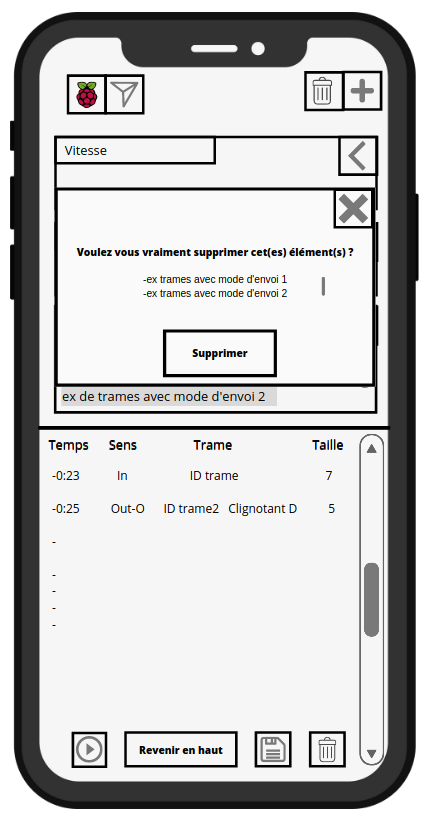
\includegraphics[width=0.45\textwidth]{sections/3_Exigences_specifiques/1_IHM/ihm/ecranSuppressionElementTrame.png}
    \captionsetup{justification=centering}
    \captionof{figure}{Affichage de PopupSuppressionElement \\ avec suppression de trames seulement}
    \label{ecran_suppression_trames}
\end{minipage} \newline
\vspace{1cm}

\newpage
\paragraph{Partie basse de l'écran}
La partie sniffer (partie basse de l'écran) présente les trames CAN envoyées et reçues par la Raspberry Pi lorsqu'il y en a. Lorsque la Raspberry Pi n'est pas encore connectée, un commentaire indique qu'il n'y a pas de trames actuellement {\guillemetleft} Pas de trame actuellement {\guillemetright} (voir figure \ref{ecran_sans_objet}). 
\newline
Les trames arrivent par le haut du terminal donc la trame la plus récente sera celle du haut. 
Pour chaque trame CAN, on précise la trame (id + donnée), l'objet auquel elle est associée (si la trame est envoyée), sa taille, son sens ({\guillemetleft} In {\guillemetright} correspond à la réception sur l'application {\nomApplication} et {\guillemetleft} Out {\guillemetright} correspond à l'émission depuis l'application {\nomApplication}) et un repère temporel. L'envoi d'une trame cyclique se remarque par l'ajout du symbole O dans son sens (Out-O).
La trame est au format {\guillemetleft} \#id\$size\@@message {\guillemetright} avec les caractères {\guillemetleft} \# {\guillemetright}, {\guillemetleft} \$ {\guillemetright} et {\guillemetleft} \@@ {\guillemetright} comme séparateurs.
\newline 
Le repère temporel est en millisecondes, et est initialisé à zéro lorsque la première trame est sniffée sur le bus CAN.
\\\\
\begin{minipage}{0.9\linewidth}
    \centering
    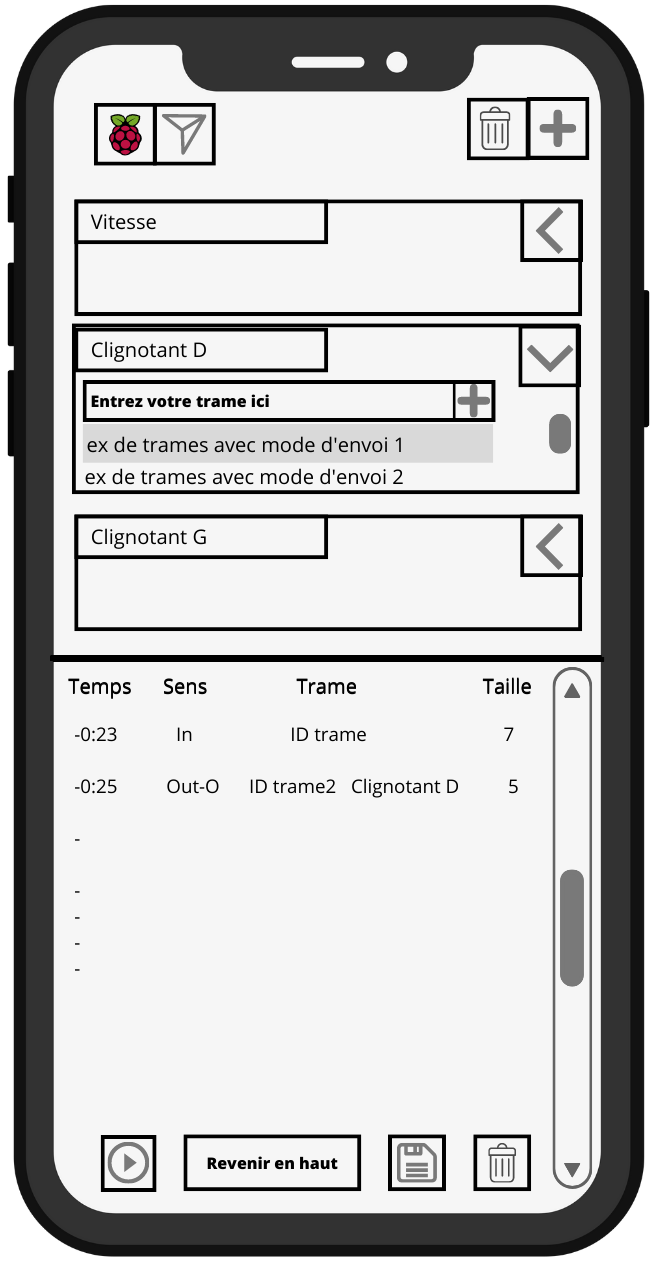
\includegraphics[width=0.45\textwidth]{sections/3_Exigences_specifiques/1_IHM/ihm/ecranPrincipalSelectionTrame.png}
    \captionof{figure}{Affichage de EcranPrincipal avec le sniffer en mode {\guillemetleft} pause {\guillemetright}}
    \label{ecran_sniffer_pause}
\end{minipage}\hfill

\newpage
Utilisateur peut mettre en pause le sniffer en cliquant sur le bouton pause (bouton [pause]) en bas à gauche de l'écran (voir figure \ref{ecran_sniffer_pause}). Lorsque le sniffer est en pause, Utilisateur peut exporter les trames présentes dans le terminal vers un fichier de log, en cliquant sur l'icône {\guillemetleft} enregistrer {\guillemetright} (bouton [exporterSniffer]) en bas à droite de l'écran. 
Il peut à la suite remettre le sniffer en écoute en cliquant sur l'icône play (bouton [play] sur la figure \ref{ecran_sniffer_pause}). Lorsque le sniffer est en cours de lecture, le bouton pour enregistrer le sniffer est verrouillé d'où le fait qu'il soit en noir sur fond gris foncé (voir figure \ref{ecran_sniffer_play}). 
\\\\
\begin{minipage}{1\linewidth}
    \centering
    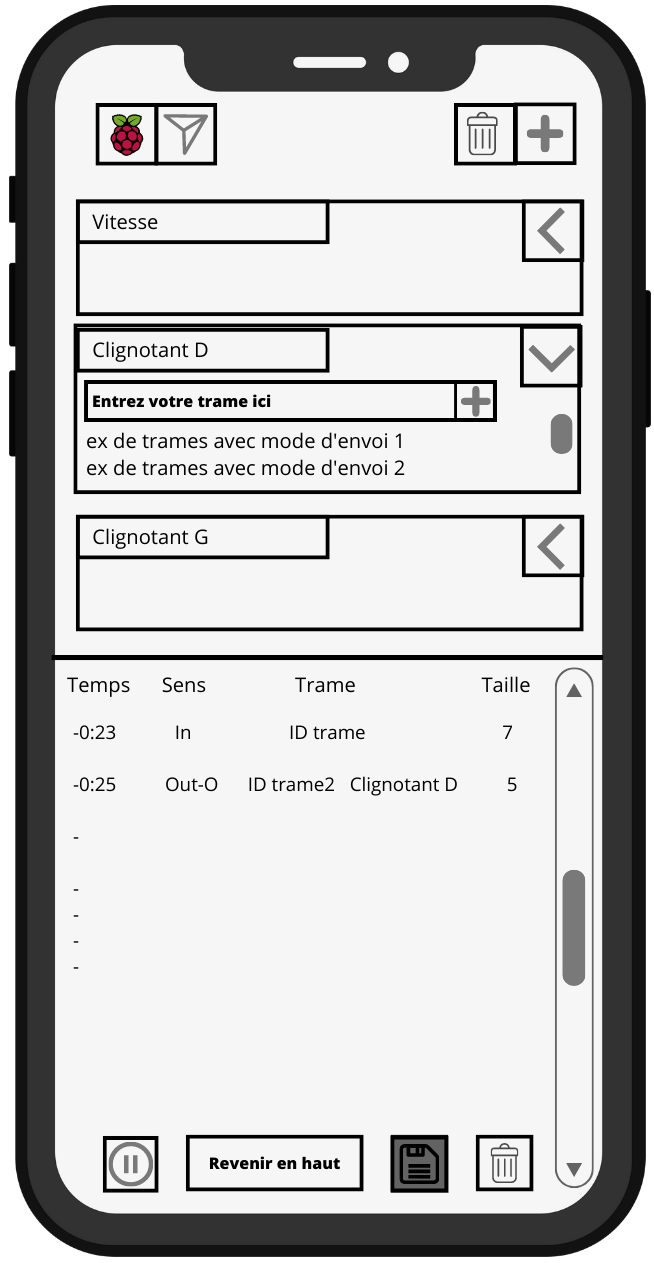
\includegraphics[width=0.4\textwidth]{sections/3_Exigences_specifiques/1_IHM/ihm/ecranSnifferPlay.png}
    \captionsetup{justification=centering}
    \captionof{figure}{Affichage de EcranPrincipal avec le \\ sniffer en mode {\guillemetleft} play {\guillemetright}}
    \label{ecran_sniffer_play}
\end{minipage}\hfill

\vspace{0.5cm}

L'enregistrement contient toutes les informations des trames visibles sur le sniffer. Les trames sont exportées dans un fichier de log (voir section \ref{dictionnaire}).\newline \\
Utilisateur peut revenir en haut de la liste des trames en cliquant sur le bouton [revenirEnHaut], et peut vider le sniffer des trames actuelles en cliquant sur la poubelle en bas de l'écran à droite sur le bouton [viderSniffer] (voir la figure \ref{ecran_sniffer_play}). 
\newpage

\subsection{Dictionnaire de domaine} \label{dictionnaire}

\begin{itemize}  
    \item \textbf{Boutons :}
        \begin{itemize}
            \item \textbf{[ajouterObjet]} : Fait apparaître PopupAjoutObjet. Permet d'ajouter de nouveaux objets. Ce bouton fait appel à la fonction ajouterObjet() de la figure \ref{schema_contexte_log}.
            \item \textbf{[ajouterTrame]} : Fait apparaître PopupModeEnvoiTrame. Permet d'ajouter une trame associée à un objet. Le bouton fait appel à la fonction ajouterTrame() de la figure \ref{schema_contexte_log}.
            \item \textbf{[annulerAjoutObjet]} :  Permet de sortir de PopupAjoutObjet. Ce bouton fait appel à la fonction refuser() de la figure \ref{schema_contexte_log}.
            \item \textbf{[annulerArretEnvoi]} : Permet d'annuler l'arrêt d'envoi de trames et de sortir de PopupArretEnvoi. Ce bouton fait appel à la fonction refuser() de la figure \ref{schema_contexte_log}.
            \item \textbf{[annulerModeEnvoi]} : Permet de sortir de PopupModeEnvoiTrame. Le nom de la trame reste cependant dans le champ de texte (<champTrame>, figure \ref{ecran_boutons}). Ce bouton fait appel à la fonction refuser() de la figure \ref{schema_contexte_log}.
            \item \textbf{[annulerReconnexion]} : Permet d'annuler la reconnexion et quitter PopupDemandeReconnexion, de manière à utiliser l'application CANdroid en mode hors connexion. Ce bouton fait appel à la fonction refuser() de la figure \ref{schema_contexte_log}.
            \item \textbf{[annulerSuppressionElement]} : Permet d'annuler la suppression des éléments sélectionnés et sortir de PopupSuppressionElement. Les éléments restent sélectionnés. Ce bouton fait appel à la fonction refuser() de la figure \ref{schema_contexte_log}.
            \item \textbf{[arreterEnvoi]} : Permet l'arrêt de l'envoi des trames en cours d'envoi. Ce bouton fait appel à la fonction arreterEnvoiTrame(mode\_envoi : booléen) de la figure \ref{schema_contexte_log}.
            \item \textbf{[connexion]} : Fait apparaître PopupDemandeReconnexion. Permet de reconnecter {\nomApplication} et {\nomLogiciel}. Ce bouton fait appel à la fonction recconecter() de la figure \ref{schema_contexte_log}.
            \item \textbf{[deplierMenuObjet]} : Permet de déplier le menu de l'objet. Ce bouton fait appel à la fonction ouvrirMenuObjet() de la figure \ref{schema_contexte_log}. 
            \item \textbf{[exporterSniffer]} : Permet d'exporter toutes les trames du sniffer dans un fichier de log. Ce bouton fait appel à la fonction exporterTramesSniffer() de la figure \ref{schema_contexte_log}.
            \item \textbf{[fermerErreurTrame]} : Permet de sortir de PopupErreurSaisieTrame. Ce bouton fait appel à la fonction quitter() de la figure \ref{schema_contexte_log}.
            \item \textbf{[fermerErreurNombreObjet]} : Permet de sortir de PopupErreurNombreObjet. Ce bouton fait appel à la fonction quitter() de la figure \ref{schema_contexte_log}.
            \item \textbf{[fermerErreurNombreTrame]} : Permet de sortir de PopupErreurNombreTrame. Ce bouton fait appel à la fonction quitter() de la figure \ref{schema_contexte_log}.
            \item \textbf{[lancerEnvoi]} : Permet d'envoyer les trames sélectionnées avec le mode ponctuel et de débuter l'envoi des trames sélectionnées avec le mode cyclique. Ce bouton fait appel à la fonction envoyerTrames() de la figure \ref{schema_contexte_log}.
            \item \textbf{[play]/[pause]} : Met en marche ou en pause le sniffer. La mise en pause fait appel à la fonction desactiverReceptionTrames(). La reprise de la lecture fait appel à la fonction activerReceptionTrames() de la figure \ref{schema_contexte_log}. 
            \item \textbf{[replierMenuObjet]} : Permet de replier le menu de l'objet. Ce bouton fait appel à la fonction fermerMenuObjet() de la figure \ref{schema_contexte_log}.
            \item \textbf{[revenirEnHaut]} : Permet de revenir en haut du sniffer. Ce bouton fait appel à la fonction revenirEnHaut() de la figure \ref{schema_contexte_log}. 
            \item \textbf{[suppressionElement]} : Fait apparaître PopupSuppressionElement. Permet de supprimer les éléments sélectionnés. Ce bouton fait appel à la fonction supprimer() de la figure \ref{schema_contexte_log}. 
            \item \textbf{[validerAjoutObjet]} : Permet de confirmer la création d'un nouvel objet et permet de sortir de PopupAjoutObjet. Ce bouton fait appel à la fonction valider() de la figure \ref{schema_contexte_log}.
            \item \textbf{[validerArretEnvoi]} : Permet de valider la demande d'arrêt d'envoi de trames et de sortir de PopupArretEnvoi. Ce bouton fait appel à la fonction valider() de la figure \ref{schema_contexte_log}.
            \item \textbf{[validerModeEnvoi]} : Permet de sauvegarder le Mode Envoi et de valider l'ajout de la nouvelle trame. Ce bouton fait appel à la fonction valider() de la figure \ref{schema_contexte_log}.
            \item \textbf{[validerSuppressionElement]} : Permet de valider la suppression des éléments sélectionnés et de sortir de PopupSuppressionElement. Ce bouton fait appel à la fonction valider() de la figure \ref{schema_contexte_log}.
            \item \textbf{[validerReconnexion]} : Permet de relancer une nouvelle procédure de reconnexion et de sortir de PopupDemandeReconnexion. Ce bouton fait appel à la fonction valider() de la figure \ref{schema_contexte_log}.
            \item \textbf{[viderSniffer]} : Permet de supprimer toutes les trames du sniffer. Ce bouton fait appel à la fonction supprimerTramesSniffer() de la figure \ref{schema_contexte_log}.\newline
        \end{itemize}
    \item \textbf{CAN} : Controller Area Network, il s'agit d'un protocole de communication série utilisé pour connecter par exemple des capteurs et des actionneurs.\newline
    \item \textbf{Champs de textes} :
        \begin{itemize}
            \item \textbf{<champNomObjet>} : Ce champ de texte correspond à la saisie du nom de l'objet. Par défaut, ce champ est pré-rempli par le Nom d'objet par défaut. Il fait appel à la fonction nommerObjet() de la figure \ref{schema_contexte_log}.
            \item \textbf{<champPeriodicite>} : Ce champ de texte correspond à la saisie de la périodicité lorsque le mode cyclique est activé. Il fait appel à la fonction saisirPeriodicite() de la figure \ref{schema_contexte_log}. 
            \item \textbf{<champTrame>} : Ce champ de texte correspond à la saisie de la trame sous le format souhaité. Il fait appel à la fonction ecrireTrame() de la figure \ref{schema_contexte_log}. \newline
        \end{itemize}
    \item \textbf{\'Ecrans utilisés} :
        \begin{itemize}
            \item \textbf{EcranPrincipal} : Affichage principal de l'application. C'est sur cet écran que Utilisateur fait la majorité de ses interactions (ajouter un objet, supprimer une trame, consulter le sniffer, etc.).
            \item \textbf{PopupAjoutObjet} : Pop-up d'ajout d'objet. Il sert à demander à Utilisateur le nom de l'objet qu'il souhaite ajouter.
            \item \textbf{PopupArretEnvoi} : Pop-up de confirmation de demande d'arrêt d'envoi de trames.
            \item \textbf{PopupDemandeReconnexion} : Pop-up de confirmation de demande de reconnexion entre {\nomApplication} et {\nomLogiciel}.
            \item \textbf{PopupErreurAjoutObjet} : Pop-up d'ajout d'objet avec le message {\guillemetleft} Vous ne pouvez pas ajouter cet objet, le nom existe déjà {\guillemetright} lorsque Utilisateur écrit un nom d'objet qui existe déjà. 
            \item \textbf{PopupErreurSaisieTrame} : Pop-up qui informe Utilisateur que le format qu'il a utilisé pour écrire la trame n'est pas le bon. PopupErreurSaisieTrame informe également sur le format à utiliser pour créer une trame.
            \item \textbf{PopupErreurNombreObjet} : Pop-up pour informer Utilisateur qu'il a atteint le nombre maximum d'objets qu'il peut créer. 
            \item \textbf{PopupErreurNombreTrame} : Pop-up pour informer Utilisateur qu'il a atteint le nombre maximum de trames qu'il peut créer.
            \item \textbf{PopupModeEnvoiTrame} : Pop-up de sélection du Mode Envoi de la trame à ajouter. Utilisateur peut choisir le mode ponctuel, ou le monde cyclique et saisir ou non la périodicité d'envoi de la trame.
            \item \textbf{PopupSuppressionElement} : Pop-up de confirmation de suppression des éléments sélectionnés. 
            \newline
        \end{itemize}
    \item \textbf{E\_Banc\_De\_Test} : Voir Tableau de Bord.\newline
    \item \textbf{E\_ICSim} : Voir Tableau de Bord.\newline
    \item \textbf{E\_PC} : Voir PC.\newline
    \item \textbf{E\_Raspberry} : Voir Raspberry PI.\newline
    \item \textbf{E\_Smartphone} : Voir Smartphone.\newline
    \item \textbf{Fichier de logs} : fichier contenant les trames du sniffer, sauvegardé sur la Raspberry Pi. Le titre du fichier est de la forme trames\_date\_heure.log.
        \begin{itemize}
            \item Date est sous la forme : JJMMAAAA (J correspond à jour, M correspond à mois, A correspond à années).
            \item Heure est sous la forme : hhmm (h correspond à heure, m correspond à minutes). \newline
        \end{itemize}
    \item \textbf{Format de la trame} : afin d'éviter à Utilisateur de taper tous les zéros non significatifs lors de la saisie d'une trame, les trames doivent être saisies avec des séparateurs de la forme suivante : 
        \begin{itemize}
            \item \#id\$size\@@message \newline
        \end{itemize}
    \item \textbf{La fin du fil} : correspond au trames reçues en dernier sur le sniffer de l'application {\nomApplication}.\newline
    \item \textbf{Nom d'objet par défaut} : Le nom par défaut est le nom donné lorsque Utilisateur ne spécifie pas de nom pour l'ajout d'un objet. Le nom par défaut sera {\guillemetleft} Objet\_ {\guillemetright} suivi de l'identifiant le plus grand déjà utilisé pour un objet, augmenté de 1. Par exemple, si les identifiants des derniers objets créés sont 10, 11 et 12, le prochain objet créé aura le nom par défaut {\guillemetleft} Objet\_13 {\guillemetright}.\newline
    \item \textbf{PC (correspond à E\_PC)} : Il s'agit d'un ordinateur fonctionnant sous Linux. Cet ordinateur dispose de Simulateur ICSim installé.\newline
    \item \textbf{Raspberry PI (correspond à E\_Raspberry)} : Ordinateur monocarte créé par la Fondation Raspberry Pi. \newline
    \item \textbf{RS485 CAN Hat} : D'après le site marchant du module (\href{https://www.waveshare.com/wiki/RS485_CAN_HAT}{https://www.waveshare.com/wiki/RS485\_CAN\_HAT}), le RS485 CAN Hat permet à une Raspberry PI de communiquer avec d'autres appareils de manière stable sur longue distance via les fonctions RS485/CAN. Dans notre cas d'utilisation, nous n'utilisons que la fonction CAN. \newline
    \item \textbf{Smartphone (correspond à E\_Smartphone)} : Téléphone portable sous système Android. \newline
    \item \textbf{Sniffer} : Un sniffer est un programme qui capture tous les paquets circulant dans le réseau. Dans notre cas, le terme sniffer est utilisé pour désigner le terminal d'affichage des trames du réseaux CAN de l'application {\nomApplication}. \newline
    \item \textbf{SSH (Secure Shell)} : Protocole sécurisé permettant une connexion distante sécurisée et des échanges de données cryptées entre un client et un serveur. SSH permet d'accéder à distance à des systèmes informatiques de manière sécurisée en utilisant des méthodes d'authentification robustes et en chiffrant les communications. \newline
    \item \textbf{Tableau de Bord}: représente l'un des (ou les) deux systèmes ci-dessous :
        \begin{itemize}
            \item \textbf{Simulateur ICSim (correspond à E\_ICSim)} : Simulateur d'un tableau de bord de voiture.
            \item \textbf{Banc de test (correspond à E\_Banc\_De\_Test)} : Banc de test d'un tableau de bord de voiture
        \end{itemize}
        Il est connecté au SàE afin d'envoyer et recevoir des trames CAN. 
        Dans tout le dossier, on emploie le terme Tableau de Bord (correspond à E\_TableauDeBord) au singulier, car le scénario nominal du SàE n'utilise que le SimulateurICSim.\newline
    \item \textbf{Types utilisés} :
        \begin{itemize}
            \item \textbf{booléen} : est un type correspondant à un booléan, c'est-à-dire soit vrai (valeur non nulle), soit faux (valeur nulle).
            \item \textbf{byte} : un ensemble de 8 bits, correspondant à l'unité de stockage d'un emplacement mémoire. C'est la plus petite unité adressable par un programme sur un ordinateur.
            \item \textbf{string} : est un type correspondant à une chaîne de caractères.
            \item \textbf{Id\_objet} : identifiant des objets.
            \item \textbf{Id\_trame} : identifiant des trames (selon leur ordre de création, donc différent de l'ID de la trame CAN).
            \item \textbf{Id\_popup} : identifiant du pop-up choisit (cf. liste des écran utilisés).
            \item \textbf{Informations} : informations visuelles visibles sur Tableau de Bord. Cela peut être un clignotant, la vitesse de la voiture, etc.
            \item \textbf{Trame} : tableau de 12 bytes.
        \end{itemize}
\end{itemize}













\label{LastPage}
\end{document}
% ------------
% FIN DOCUMENT 
% ------------